\documentclass[letterpaper, spanish, 11pt]{report}
%\renewcommand{\baselinestretch}{1.5}
\usepackage{setspace}
\usepackage[letterpaper, margin=2.5cm]{geometry}
\usepackage[spanish]{babel}
\usepackage{graphicx}
\graphicspath{ {images/} }
\usepackage{booktabs}
\usepackage{multirow}
\usepackage{listings}
\usepackage{color}
\usepackage{amsmath}
\usepackage{float}
\definecolor{mygreen}{rgb}{0,0.6,0}
\definecolor{mygray}{rgb}{0.5,0.5,0.5}
\definecolor{mymauve}{rgb}{0.58,0,0.82}

\lstset{ %
  backgroundcolor=\color{white},   % choose the background color
  basicstyle=\footnotesize,        % size of fonts used for the code
  breaklines=true,                 % automatic line breaking only at whitespace
  captionpos=b,                    % sets the caption-position to bottom
  commentstyle=\color{mygreen},    % comment style
  escapeinside={\%*}{*)},          % if you want to add LaTeX within your code
  keywordstyle=\color{blue},       % keyword style
  stringstyle=\color{mymauve},     % string literal style
}

\selectlanguage{spanish}
\usepackage[utf8]{inputenc}
\setcounter{secnumdepth}{0}
\usepackage{titlesec}
\titleformat{\chapter}[display]{\normalfont\bfseries}{}{0pt}{\Huge}
\usepackage{lipsum}
\addto\captionsspanish{\renewcommand{\bibname}{Referencias}}
\renewcommand{\bibname}{Referencias}
\usepackage{helvet}
\renewcommand{\familydefault}{\sfdefault}
\usepackage{caption}
\captionsetup{font=footnotesize}

\usepackage{fancyhdr}
\fancyhf{} % clear all header and footers
\renewcommand{\headrulewidth}{0pt} % remove the header rule
\rhead{\thepage}
\pagestyle{fancy}

\pagestyle{myheadings}
\makeatletter
\def\@oddhead{{\slshape\rightmark}\hfil\footnotesize\thepage}%
\makeatother

% new packages in Marco Teorico, please copy on total thesis work
\usepackage{amsmath}
\DeclareMathOperator*{\argmax}{argmax} % thin space, limits underneath in displays
\DeclareMathOperator*{\argmin}{argmin} % thin space, limits underneath in displays
\usepackage[hyphens,spaces]{url}
\usepackage{listings} %For code in appendix
\lstset
{ %Formatting for code in appendix
    language=R,
    basicstyle=\footnotesize,
    numbers=left,
    stepnumber=1,
    showstringspaces=false,
    tabsize=1,
    breaklines=true,
    breakatwhitespace=false,
}
\usepackage{booktabs}
\usepackage{adjustbox}
\usepackage{graphicx}
\pagenumbering{roman}

\begin{document}

\begin{titlepage}
\begin{center}
\vspace*{1cm}    


\includegraphics[width=0.6 \textwidth]{logoubj.png} \\
\large{Universidad Benito Juárez G.}

\vspace{3cm}
\textbf{Ariel Estanislao Meilij Ezeiza}

\vspace{3cm}
\huge
Modelo Predictivo de la Tasa Representativa de Mercado de Colombia Utilizando Aprendizaje Automatizado

\vspace{3cm}
\large
\textbf{Tesis para obtener el grado de Doctor en Administración Gerencial}

\vspace{4cm}
\small
\textit{Julio 14 del 2018}

\end{center}
\end{titlepage}

\pagenumbering{gobble}

\Large
 \begin{center}
Resumen\\ 
\hspace{5pt}

% Author names and affiliations
\large
Ariel E. Meilij$^1,^2$  \\
\hspace{5pt}

\small  
$^1$) Universidad Benito Juárez G.\\
ariel.meilij@gmail.com\\
$^2$) Universidad Latinoamericana de Ciencia y Tecnología
\end{center}
\hspace{5pt}

\normalsize
El siguiente trabajo de investigación tiene como finalidad determinar un modelo de predicción para la tasa de cambio del dólar en Colombia (conocida legalmente como la TRM) utilizando aprendizaje automatizado. La investigación se enfoca en la hipótesis de que las series de tiempo pueden utilizarse como elementos de predicción por contener la tendencia de una variable, pero son más fuertes cuando se utilizan las variables exógenas que modelan e intervienen en dicho comportamiento. Para la TRM estas variables independientes son los regresores representados por los principales rubros de exportación del país. En vez de extraer un modelo en base a la observación, se utiliza el aprendizaje automatizado para entrenar los datos de las series de tiempo de la TRM y los rubros de exportación, y se unen con un modelo ensamblado de pronostico ARIMA para la serie de tiempo y regresión multivariable para los factores exógenos. 

\hspace{10pt}

\Large
 \begin{center}
Abstract\\ 
\hspace{5pt}
\end{center}

\normalsize
The following research thesis objective is the determination of a prediction model for the Colombian Peso exchange rate (legally known as the TRM) using machine learning techniques. The research focuses on the hipothesis that time series can be used for forecasting purposes given their intrinsic trend capacity, but their potential can be strengthened when coupled with exogenous variables that confound said behavior. For the TRM these independent variables are represented by the principal export components. Instead of extracting a model through observation, machine learning is used to train the different time series representing the values of the TRM and exports. Ensambled methodologies of stacking are then used to join the predictive capacities of ARIMA forecasting for TRM time series and multivariable regresion for the different export variables confounding the TRM pricing.
\clearpage
\begin{center}
    \thispagestyle{empty}
    \vspace*{\fill}
        Existen pocas metas en la vida profesional y académica de una persona como la investigación científica que implica el doctorado. Más allá de la dedicación personal, el esfuerzo de superación o la curiosidad humana que trata de abarcar un poco más de lo que se puede ver, entender o explicar, existe un cúmulo de personas que sacrifican su tiempo y aportan una cuota mayor de paciencia que el mismo doctorando. Todas estas personas fueron, son y serán el punto de apoyo para todos los empréstitos pasados, este en particular, y todos los proyectos futuros que puedan devenir. Por esa misma razón, estoy dedicando la siguiente tesis doctoral a las personas que la han hecho realidad.
            
        \begin{itemize}
            \item Primero que nada a mi esposa Ángela Alejo, quien ha sido la piedra angular de todo lo que soy y todo lo que seré en el futuro. 
            \item A nuestra hija Ruth Meilij, futura Física Cuántica, y una de las tantas (pocas) personas que entiende de \LaTeX y FORTRAN.
            \item A mis padres Norma Ezeiza y Ricardo Meilij, quienes siempre creyeron que lo lograría y sacrificaron muchos fines de semana para que pudiera estudiar.
            \item A mi jefe Max Harari por prestarme un libro de Big Data en el 2014 y despertar la curiosidad por la Ciencia de Datos. Siempre quise ser un Data Scientist, simplemente no sabía que existía tal cosa hasta que un libro me dejó más preguntas que respuestas. 
            \item A los profesores Roger Peng, Ph.D., Jeff Leek, Ph.D. y Brian Caffo, Ph.D. de \emph{Johns Hopkins University}. Gracias a sus clases y emprendimiento aprendí las habilidades de estadística, programación y matemáticas que me permitieron seguir investigando. 
            \item A los increíbles profesores de la Universidad Benito Juárez G. Es poco probable que entiendan la importancia y evolución que significan para todos los doctorandos del grupo G2V2. Por eso es tan importante que sepan que se está sembrando en estos momentos la nueva generación de investigadores del área de la Administración Gerencial en Latinoamérica gracias a sus esfuerzo. 
        \end{itemize}
    \vspace*{\fill}
    \end{center}
\clearpage

\tableofcontents
\listoffigures
\listoftables
\begin{spacing}{1.5}
\pagenumbering{roman}
\setcounter{chapter}{-1}
\chapter{Introducción}
\thispagestyle{empty}

\section{Antecedentes de la Investigación}
Para todas las empresas que importan producto para su comercialización en el territorio de Colombia, el manejo de la TRM es uno de los problemas mayores que deben confrontar. La tasa de cambio representativa del mercado (TRM por sus siglas) es el valor en pesos colombianos que una empresa tiene que desembolsar por un dólar estadounidense. A pesar que no todas las importaciones provienen de Estados Unidos, inclusive aquellas que se realizan con Asia tienen facturación en dólares. De aquí que el dólar sea tan ubicuo en los procesos de comercio internacional, que Colombia como país importador y exportador haya tenido que crear una figura legal solamente para esta razón entre dos monedas. 

La TRM afecta una serie de variables dentro del proceso comercial de una empresa. 

\begin{itemize}
	\item Las listas de precios que emita el departamento de contabilidad estarán sujetas a la TRM en curso. Si el departamento de finanzas e importación no realizó la mejor negociación de la TRM, los precios se verán afectados de manera negativa, ya que su costo es mayor por afectación directa del cambio de dólares americanos a pesos colombianos.
	\item El departamento de ventas tendrá un especial interés en evitar las fluctuaciones constantes de listas de precio, que inevitablemente el departamento de contabilidad actualizará, si no puede prever la variación misma de la TRM en un horizonte de corto a mediano plazo. 
	\item Asimismo, el departamento de mercadeo vigilará de cerca que la variación de precios sea mínima, ya que la variable precio es una de las 4 P’s de la ciencia de la mercadotecnia (siendo todas posicionamiento, precio, producto y publicidad). La variación del precio al alza aliena a los consumidores, que pueden no ver la razón de la misma en el aumento de la TRM sino en la mala fe del importador. 	
\end{itemize}

Para protegerse de los efectos de la variación de la moneda, las empresas algunas veces recurren al concepto de forwards, o contratos de compras a futuros de moneda extranjera pactados a un precio dado que reduce el margen de incertidumbre. Dentro de la contabilidad moderna, y aplicado a la importación de productos, el contrato de forward es un elemento de costeo. Con esto la empresa puede asignar costos a un producto a un valor dado de tasa de cambio el cual es conocido y no sufrirá variación. Esto no implica que sea el mejor valor o el mejor negociado, solo que el precio final al momento de ejecutarse el contrato no sufre variación y no hay incertidumbre sobre el mismo. 

Muchas empresas no efectúan contratos de compra de moneda a futuro haciendo acuso del carácter especulativo de los mismos. El horizonte de planificación de un importador involucra un ciclo de noventa a ciento veinte días en el cual factura y cobra sus ventas a crédito. Dentro de ese plazo, es probable que la TRM haya reducido por debajo del valor pactado en el contrato futuros, incurriendo en gastos innecesarios por reducir la incertidumbre del cambio. Otras empresas solo cubren una porción del valor total de la operación con contratos futuros tratando de optimizar el resultado de la misma y perder el menor margen posible de rentabilidad versus el costo de cobertura. 

El problema mayor para todas estas empresas es poder predecir con algún valor matemático y científico cuál será el valor de la TRM en cualquier momento dado. Existe en la comunidad financiera - y en la comunidad de comerciantes en general - una idea acertada de que la TRM está relacionada a los movimientos del precio internacional del petróleo, principal producto de exportación de Colombia, y por ende, el mayor contribuyente a estabilizar la balanza de pago del país y la necesidad de equilibrar los flujos de moneda internacional con las reservas nacionales. Estos estudios incluyen los reportes de casas financieras importantes como J. P. Morgan, las cuales han analizado las fluctuaciones de la cesta petrolera y la TRM hasta un índice de correlación cercano al 70 por ciento (o en términos matemáticos, un coeficiente de correlación \(R^{2} ~ 0.7\) ). 

Para el estadista entrenado, un índice de correlación \(R^{2}\) de 0.7 en un buen indicio de correlación, pero lejos de un valor que pueda completar un modelo de predicción. Para la ciencia de datos, es sin embargo un comienzo prometedor de un modelo predictivo en potencia que puede construirse a través de las nuevas metodologías de Aprendizaje Automatizado. El aprendizaje automatizado utiliza técnicas matemáticas y de estadística avanzadas para aprender de los datos históricos y crear modelos de predicción altamente confiables. El aprendizaje automatizado no es inteligencia artificial (aunque la inteligencia artificial usa aprendizaje automatizado), sino que es el conjunto de herramientas de la ciencia de datos que hoy ayuda a diseñar teclados que predicen el texto, motores de búsqueda en Internet, autos que se manejan solos, y búsqueda de solución a enfermedades como el cáncer. 

¿Hay una manera más eficaz de poder modelar y predecir la TRM para minimizar los efectos negativos de las variaciones de la misma en la comercialización de productos importados? ¿Hay otros elementos además de la cesta de petróleo que jueguen un papel determinante en la fijación del valor de la TRM? ¿Si la Superintendencia sólo mide el valor en base al intercambio de compradores y vendedores, como juegan estos dos en la fijación del precio si son solo agentes secundarios de procesos de importación y exportación?

Una empresa que cuente con el conocimiento y tecnología para poder predecir y proyectar el valor de la TRM podrás reducir el impacto negativo en el proceso de comercialización mientras que optimiza el rendimiento financiero en sus áreas contables. 

\section{Objetivo general}
El objetivo principal de la investigación es construir un modelo parsimonioso predictivo que permita determinar el valor futuro de la TRM a partir de variables predictivas dadas.

\subsection{Objetivos específicos}
Los objetivos específicos de la investigación son los siguientes:

\begin{itemize}
	\item Identificar que variables dentro del marco económico colombiano son las que tienen mayor grado de incidencia en la determinación de la TRM colombiana. 
	\item Cuantificar cuales y cuantas de estas variables forman parte de un modelo predictivo parsimonioso que permita realizar predicciones dentro de un intervalo de confidencia con valores de p = 0.05. 
	\item Determinar qué tipo de modelo parsimonioso es el correcto utilizando las variables predictivas del punto anterior con los mismos intervalos de confidencia, o en su defecto si este es un modelo predictivo compuesto. 
\end{itemize}

\section{Justificación de la investigación}
La justificación de dicha investigación está basada en el costo que afrontan las empresas que no pueden determinar exactamente el valor de la TRM dentro de su ciclo operativo anual e incurren en pérdidas dadas por:

\begin{enumerate}
	\item Falta de ventas al costear incorrectamente sus productos por encima del valor de mercado
	\item Perdidas contables al costear incorrectamente sus productos a valor del mercado y luego verificar que no están cubiertas las deudas en moneda extranjera y que la TRM tiene un valor superior al utilizado
	\item Perdidas contables en los contratos futuros de compra de divisas con los bancos en el cual el precio de ejecución termina siendo superior al valor actual de la TRM (en dicho caso, para el banco es una operación altamente rentable)
\end{enumerate}

Adicionalmente, la siguiente investigación plantea el uso de una metodología relativamente nueva en el campo de la administración como lo es el aprendizaje automatizado. La ciencia de datos es una disciplina principalmente multidisciplinaria, que recién ahora comienza a tener alguna participación oficial en algunas universidades del mundo. El enfoque ha sido utilizado con éxito en la ingeniera y ciencias de la computación, así como en la bioestadística, pero es muy poco su uso académico en las ciencias administrativas y financieras, por lo que el enfoque es novedoso y abre las puertas a la resolución de muchos más problemas con una metodología cuantitativa similar.

\section{Alcances y Limitaciones}
Las siguientes son los alcances y limitaciones de la investigación. 

\begin{itemize}
	\item El siguiente estudio está basado en la TRM colombiana, que por su propia definición establece una razón entre dos divisas, el peso colombiano y el dólar estadounidense. Aun cuando la solución prevista al problema muy probablemente pudiera utilizarse con otras monedas, esta investigación no las abarca.
	\item El siguiente estudio no hace referencia ni analiza en profundidad el sistema para determinar la TRM por parte de la Superintendencia Financiera de Colombia; este pudiera ser un tema interesante de tesis de posgrado para un futuro investigador. El resultado final del método de la Superintendencia Financiera de Colombia para el valor de la TRM se utiliza solo como una observación matemática de un hecho predecible a partir de ene cantidad de variables. 
	\item El siguiente estudio utiliza base de datos y datos oficiales históricos medidos desde el año 2000 hasta el año 2017. Si bien este valor es menor al de una generación, ha sido arbitrariamente establecido como punto de quiebre ya que reúne muchos más datos estadísticos de los necesarios para un modelo predictivo de gran precisión. 
	\item La siguiente investigación busca un modelo predictivo parsimonioso. Un modelo parsimonioso en estadística es un modelo que cumple con el valor predictivo buscado con el menor número de variables predictivas necesarias. Puede entonces existir variables predictivas que afecten el valor de la TRM pero que este estudio no incluirá si el resultado del modelo predictivo es suficiente con un número menor de variables.
\end{itemize} 
\end{spacing}
\pagenumbering{arabic}
\setcounter{chapter}{0}
\chapter{Capítulo I: \\Protocolo de Investigación}
\thispagestyle{empty}

\section{El Problema de Investigación}
El siguiente proyecto de investigación busca analizar el problema de la determinación del valor futuro de la TRM de Colombia en base a los componentes principales de exportación del país, que conforman su cesta de divisas, con miras a crear un modelo predictivo matemático que le sirva a la organización para la optimizar los procesos comerciales y financieros de la misma. ¿Qué es la TRM que afecta tanto el funcionamiento de los importadores? Actualmente la Superintendencia Financiera de Colombia es la que calcula y certifica diariamente la TRM con base en las operaciones registradas el día hábil inmediatamente anterior y la define de la siguiente manera (Circular Reglamentaria Externa del Banco de la República DODM-146, 2015):

\begin{quotation}
	La tasa de cambio representativa del mercado (TRM) es la cantidad de pesos colombianos por un dólar de los Estados Unidos (antes del 27 de noviembre de 1991 la tasa de cambio del mercado colombiano estaba dada por el valor de un certificado de cambio). La TRM se calcula con base en las operaciones de compra y venta de divisas entre intermediarios financieros que tranzan en el mercado cambiario colombiano, con cumplimiento el mismo día cuando se realiza la negociación de las divisas.
\end{quotation}

La Superintendencia Financiera de Colombia no determina el valor de la TRM sino de un elemento derivado de las operaciones de compra y venta de la misma. Son los agentes de operación (exportadores que venden sus productos en dólares y los deben canjear a pesos colombianos e importadores que compran sus productos en dólares y para tal fin cambian sus pesos colombianos). Ambos obedecen a fuerzas del mercado que dan forma y materializan la valorización. 

Es de conocimiento que la cesta petrolera influye en la valorización de la TRM, sin embargo, poco o nada se ha estudiado de que otras variables actúan en la ecuación total. Cada una de estas debe pensarse como una variable independiente de un modelo predictivo que interviene en la valorización total de la TRM, y sin los cuales la formula queda incompleta.

\section{Impacto Social}
El trabajo cumple con la dimensión de relevancia social. Ninguna empresa quiere costear sus productos por encima de los demás agentes del mercado, so pena de perder participación de mercado a sus competidores con precios más ventajosos. La capacidad de estimar a futuro el mejor pronóstico de tasa de cambio reduce el porcentaje de carga por previsión de volatilidad de moneda (también conocido en contabilidad como colchón) lo que redunda en un precio mejor para el consumidor y la sociedad en general. Al reducir las ineficiencias del cálculo de costos prediciendo de forma correcta la tasa de cambio los consumidores ganan el diferencial entre el precio pobremente estimado y un precio ajustado a las realidades del cambio futuro.

\section{Línea de Investigación}
El siguiente trabajo de investigación se apega a la línea de investigación financiera de la UBJ. La universidad define la línea financiera como aquella que investiga modelos económicos y financieros innovadores que impulsen el crecimiento y sustentabilidad de la organización a fin de relevar su competitividad \cite{guiaAcademicaDAG}. 

La hipótesis de trabajo de la investigación propone un nuevo modelo de predicción de la tasa de cambio de Colombia utilizando aprendizaje automatizado y un modelo ensamblado de aprendices, lo que representa un enfoque innovador para mejorar la situación de optimización de costos y competitividad de la empresa. 

\section{Tipo de Estudio}
El tipo de estudio es hipotético deductivo, cuantitativo.

Es hipotético deductivo porque:

\begin{itemize}
\item Partimos de una teoría base (macroeconomía que sustenta la tasa de cambio con la balanza de pagos y exportaciones, machine learning para deducir modelos predictivos en base a grandes muestras de datos) 
\item Formulamos una hipótesis de trabajo
\item Aplicamos ciencia de datos para una recolección masiva de datos de diferentes regresores (cada uno un rubro importante de exportaciones de Colombia)
\item Confirmamos la hipótesis al extraer un modelo predictivo estadístico  
\end{itemize}

\section{Pregunta de Investigación}
La pregunta de investigación de este anteproyecto surge de una pregunta real y de aplicación necesaria en el ámbito empresarial de una organización importadora de bienes de consumo masivo al mercado de Colombia: \emph{¿Cómo podemos predecir la TRM para mitigar el efecto negativo de las fluctuaciones en la tasa de cambio en la contabilidad de precios y costos?}

\section{Objetivo General de la Investigación}
El objetivo principal de la investigación es construir un modelo parsimonioso predictivo que permita determinar el valor futuro de la TRM a partir de variables predictivas dadas.

\subsection{Objetivos específicos}
Los objetivos específicos de la investigación son los siguientes:

\begin{itemize}
	\item Identificar que variables dentro del marco económico colombiano son las que tienen mayor grado de incidencia en la determinación de la TRM colombiana. 
	\item Cuantificar cuales y cuantas de estas variables forman parte de un modelo predictivo parsimonioso que permita realizar predicciones dentro de un intervalo de confidencia con valores de p = 0.05. 
	\item Determinar qué tipo de modelo parsimonioso es el correcto utilizando las variables predictivas del punto anterior con los mismos intervalos de confidencia, o en su defecto si este es un modelo predictivo compuesto. 
\end{itemize}

La intención del trabajo de investigación es integrar el uso de rubros de exportación como series de tiempo para el entrenamiento de modelos de aprendizaje automatizado en forma de aprendices. La determinación del modelo no la hace el investigador sino que la metodología de aprendizaje automatizado ayuda a entrenar los datos para extraer el modelo. Uno o ambos de estos modelos debe cumplir con la premisa de alcanzar un alto nivel de predicción. Si ambos modelos cumplen con la premisa de alto valor predictivo entonces sus egresos - los valores estimados - serán utilizados como entradas de un tercer modelo ensamblado (conocido en inglés como modelo apilado o \textit{stacking}) para diseñar un modelo predictivo parsimonioso final con mayor valor de precisión.   

\section{Alcances y Limitaciones}
Las siguientes son los alcances y limitaciones de la investigación. 

\begin{itemize}
	\item El siguiente estudio está basado en la TRM colombiana, que por su propia definición establece una razón entre dos divisas, el peso colombiano y el dólar estadounidense. Aun cuando la solución prevista al problema muy probablemente pudiera utilizarse con otras monedas, esta investigación no las abarca.
	\item El siguiente estudio no hace referencia ni analiza en profundidad el sistema para determinar la TRM por parte de la Superintendencia Financiera de Colombia; este pudiera ser un tema interesante de tesis de posgrado para un futuro investigador. El resultado final del método de la Superintendencia Financiera de Colombia para el valor de la TRM se utiliza solo como una observación matemática de un hecho predecible a partir de ene cantidad de variables. 
	\item El siguiente estudio utiliza base de datos y datos oficiales históricos medidos desde el año 2000 hasta el año 2017. Si bien este valor es menor al de una generación, ha sido arbitrariamente establecido como punto de quiebre ya que reúne muchos más datos estadísticos de los necesarios para un modelo predictivo de gran precisión. 
	\item La siguiente investigación busca un modelo predictivo parsimonioso. Un modelo parsimonioso en estadística es un modelo que cumple con el valor predictivo buscado con el menor número de variables predictivas necesarias. Puede entonces existir variables predictivas que afecten el valor de la TRM pero que este estudio no incluirá si el resultado del modelo predictivo es suficiente con un número menor de variables.
\end{itemize} 

\setcounter{chapter}{1}
\chapter{Capítulo II: \\Fundamento Teórico}
\thispagestyle{empty}

\section{Estado del Arte}
A pesar de ser un campo relativamente nuevo, la Ciencia de Datos está profundamente sustentada por la teoría académica (quizás por sus implicaciones como campo multidisciplinario y su importancia para la solución de problemas que impactan otras disciplinas).

De acuerdo a la bibliografía existente, la primera persona en hacer un bosquejo de la idea fue el académico Danés Peter Naur en su libro “Concise Survery of Computer Methods”. Naur sin embargo utiliza el término más que nada para sustituir el de ciencia computacional \cite{naur}. El investigador de Laboratorios Bell y profesor de la Universidad de Princeton, John Tukey, hace un mejor acercamiento al escribir el primer artículo científico sobre como la disciplina de la estadística cambiaba con el advenimiento de la informática \cite{tukey}. Mucho más tarde fue el estadista de la Universidad de Tokio Chikio Hayashi quien definiría de manera sucinta el concepto de Ciencia de Datos como un concepto sintético para unificar la estadística, el análisis de datos y los métodos relacionados con la consecución lo resultados \cite{hayashi}.

Es interesante que los métodos de aprendizaje automatizado proliferaron de forma paralela al concepto de ciencia de datos, y solo fueron absorbidos por esta en los últimos diez años. Alpaydim nos describe el aprendizaje automatizado como la programación de computadoras para optimizar un criterio de desempeño utilizando datos o experiencia pasada \cite{alpaydin}. Tom Mitchell respeta este concepto al describir el aprendizaje automatizado como “… la construcción de programas computacionales que aprenden con la experiencia…” \cite[pag. XV]{mitchell}. Solo Peter Harrington utiliza una descripción mucho más simplista al determinar que “El aprendizaje automatizado es la extracción de información de la data.” \cite[pag. 5]{harrington}.

La teoría detrás de la regresión lineal es bastante homogénea a través de todos los autores. Zumel y Mount describen la regresión lineal como el más común de los métodos de aprendizaje automatizado \cite{zumelMount}, y si no, es muy fácil verificar cual otro método probar como segunda opción. Para Daroczi, el énfasis está en los modelos de regresión multivariable (una extensión de la regresión lineal simple de un solo predictor y resultado) que construyen el camino para la predicción de fenómenos complejos en la naturaleza y negocios \cite{daroczi}. Por su parte, Harrington resume los beneficios de la regresión lineal \cite{harrington} por la facilidad de interpretar los resultados y lo frugal en el uso de ciclos de computación (aunque puede ser menos útil si el fenómeno no es perfectamente lineal).
 
Muchos autores han escrito sobre las series de tiempo, pero es difícil agregar al tema o discutir las ideas del profesor Robert Hyndman, uno de los expertos más respetados en la comunidad de la estadística por su trabajo en las series de tiempo. Hyndman extiende la teoría a las series de tiempo como elementos de pronóstico y su relación con la regresión lineal \cite{hyndman}. Desde el punto de vista técnico, Hyndman es el creador de varias bibliotecas de funciones de pronóstico utilizando series de tiempo y ARIMA en lenguaje R. Dentro de la bibliografía, Daroczi es quien agrega detalles sobre la detección temprana de valores atípicos que pueden dificultar – y mucho – el análisis \cite{daroczi}. Un componente importante de las series de datos es la detección de si son o no auto-regresivas (lo que determina mucho de su poder predictivo). La fórmula para la detección de series auto-regresivas es el test Dickey-Fuller, y la mejor bibliografía es el artículo científico escrito por ambos profesores en la revista especializada Econometrica \cite{dickeyfuller}. A pesar de ser un artículo contemporáneo, la teoría detrás de la prueba Dickey-Fuller nos permite descartar series de tiempo no-regresivas con poco poder de predicción.
 
El uso de modelos ensamblados es en cierta forma la prueba final de la hipótesis de trabajo: la utilización de dos modelos entrecruzados cuyos resultados conforman una tabla temporal de valores esperados de los cuales se genera un nuevo modelo sintético de predicción más general y con mayor capacidad de predicción en juegos de datos de validación cruzada. Este concepto es novel; Witten y Frank lo describen como combinación de métodos múltiples, y escriben: “… un enfoque obvio para hacer mejores decisiones es tomar el resultado de diferentes métodos y combinarlos…” \cite{datamining}. Zhou nos describe que “… los modelos ensamblados que entrenan múltiples variables y luego las combinan para uso de entrenamiento, con el Boosting y el Bagging como representantes principales, representan lo más novedoso en el estado del arte de la ciencia de datos…” \cite[pag. 5]{ensembleMethods}. De una manera un tanto más coloquial, Zhang y Ma describen el uso de modelos ensamblados con una analogía de la vida real, en la cual los pacientes buscan una segunda y hasta tercera opinión de expertos antes de someterse a una operación complicada \cite{ensembleMachineLearning}. Curiosamente tanto Zhang, Ma y Zhou hablan de la combinación de métodos de regresión general con clasificadores, y solo Witten y Frank hablan de otras combinaciones (por supuesto, Witten y Frank comenzaban a escribir en los albores del ensamblaje de métodos, cuando los clasificadores no estaban tan de moda porque el análisis era mayoritariamente de números, algo que cambió con el avance de las redes sociales).

En su libro “Crisis Cambiarias en Países Emergentes” el Dr. Bernardo Carriello utiliza un modelo de descripción (más que de predicción) de corrida de las tasas de cambios, en el cual los regresores incluían variables de medición económicos como crédito privado como porcentaje del PIB, tasa de variación de reservas, desalineación de tipo real, y otros \cite{crisisCambiarias}. Carriello utiliza muchísimo modelos lineales dicotómicos que modelan los escenarios con variables binarias (algo muy común entre los economistas) que por lo general favorecen regresiones logísticas o con la utilización de variables dummy o comodín (se multiplican por el coeficiente uno o cero según tengan o no valor). La mayoría de la bibliografía de aprendizaje automatizado y ciencias de datos prefieren el estudio de variables continuas y reales con amplitud de rango y valores, algo que está más cerca de la disciplina de la bioestadística que de la economía. Una pregunta adicional válida es si tomar metodologías más cercanas a la bioestadística se aplica para la predicción financiera mejor que los modelos dicotómicos actuales.
 
Volviendo a la pregunta mayor de área, el autor y antiguo Ministro de Economía de Colombia, Alfonso Ortega Cárdenas, menciona como material de bibliografía universitaria, la re-valorización del dólar frente al peso colombiano tras el comienzo de la caída de los precios del petróleo a partir del año 2015 \cite{cardenas}. El Dr. Cárdenas no hace mucho hincapié en la correlación de ambas variables, y prefiere ahondar en temas macro-económicos como la variación de la tasa de interés como elemento de presión en la tasa cambiaria y las leyes de ingreso de capital extranjero. Pero es claro que el efecto de las fuentes de ingreso del petróleo como variable clave en el valor final de la TRM ya han sido definidas – si bien algo ligeramente – como claves en un libro de texto de economía de Colombia. ¿Hay elementos adicionales que indiquen la importancia de otras fuentes de ingresos como posibles modeladores y variables de predicción de la TRM? Si los hay, y aparecen en la misma bibliografía de Cárdenas quien describe en detalle a) el sector petrolero, b) el sector siderúrgico, c) el carbón, y d) el níquel.

Los autores Castaño, Callejas, Ochoa y Henao de la Facultad de Ciencias Económicas de la Universidad de Antioquia, hacen un trabajo innovador y de avanzada técnicas estadísticas en su artículo científico \emph{Modelando el Esquema de Intervenciones del Tipo de Cambio para Colombia}. En dicho escrito se determina la eficiencia de las intervenciones realizadas por el Banco de la República empleando el modelo teórico del canal de coordinación. Los autores evalúan el efecto que tiene el diferencial de tasas de interés, la variable de intervenciones construida por medio de un modelo \emph{Markov-switching}, y el procedimiento de inversionistas técnicos y fundamentalistas sobre diferentes cuantiles del retorno de la tasa representativa del mercado (TRM). La metodología utilizada son las regresiones de cuantiles bajo redes neuronales \cite{modelandoIntervenciones}. Castaño, Callejas, Ochoa y Henao no son los únicos en utilizar redes neuronales, o una variante de redes neuronales, para entrenar modelos de predicción. Los profesores de la Universidad de Parana, Brasil, Scarpin y Steiner utilizan un modelo de Redes Neuronales Radiales Artificiales para un modelo de pronóstico de reemplazo de artículos vendidos en supermercados \cite{scarpinSteiner}. Sin embargo el modelo propuesto por Scarpin y Steiner necesita alimentarse no solo de la data actualizada de movimientos de producto, sino de un pronóstico inicial de necesidades de niveles de venta. Con una base similar - la necesidad de un pronóstico a priori - pero una metodología diferente, los doctores Wang y Xu crean un marco para pronosticos cooperativos utilizando modelos basados en Pronósticos Combinados de Bayes \cite{wangXu}. 
 
Los investigadores Mehreen Rehman, Gul Muhammad Khan y Sahibzada Ali Mahmud han utilizado la ciencia de datos para la predicción de FOREX. Los autores utilizan CGP (Programación Genética Cartesiana), una extensión del uso de redes neuronales, para obtener predicciones del dólar australiano con 98.72\% de precisión por períodos extendidos de hasta 1,000 días \cite{rehmanKhanMahmud}. Los autores alimentan el sistema CGP con información histórica de las monedas en cuestión compuesta por 500 días de cotización.
 
Quizás menos conocido es el uso de clasificadores versus regresores. Este camino toma el estudio de los doctores Hossein Talebi, Winsor Hoang y Marina Gavrilova. En su investigación en búsqueda de la mejora de sistemas automatizados de corretaje de FOREX utilizando aprendizaje automatizado, los autores proponen un nuevo método de clasificación. Dicho método utiliza extracción de clasificadores de múltiples escalas para el entrenamiento de datos, y luego se ensamblan diferentes clasificadores por voto Bayes \cite{talebiHoang}. El método propuesto demuestra superioridad a la hora de ensamblar clasificadores por encima de clasificadores individuales.
 
Otro estudio interesante es el de los profesores de matemática de la universidad de Beijing Lean Yu, Shouyang Wang, y K. K. Lai. El enfoque es novedoso en el sentido que utilizan un sistema ensamblado de auto-regresión lineal generalizada (GLAR) con redes neuronales artificiales (ANN). Los autores llegan a la conclusión que los resultados en las predicciones son superiores a los resultados de las predicciones de los métodos por separado, o de métodos similares con regresiones lineales \cite{yuWangLai}. Una lectura cuidadosa de los resultados evidencia márgenes de error del 1.56\% al 3.57\%, dependiendo de la moneda a evaluar.

\section{Marco Teórico}
La Ciencia de Datos se caracteriza por ser una ciencia multidisciplinaria. A la par de extenso conocimiento de estadística y programación, el científico de datos debe poseer un dominio extremo sobre el campo de acción o \textit{domain expertise} como se le conoce en inglés \cite{pengMatsui}. Este portafolio de conocimiento se refleja de igual manera en el marco teórico del trabajo de investigación, que debe unir, analizar y sintetizar la teoría de la estadística descriptiva e inferencial, el aprendizaje automatizado y los modelos ensamblados para la resolución del problema, y la economía de Colombia para entender el problema en toda su magnitud. Por tales razones se ha decidido desglosar el marco teórico en seis secciones diferentes, cada una con su base de conocimiento distintivo. 

\begin{enumerate}
    \item La Economía de Colombia
    \item Regresión Lineal
    \item Series de Tiempo
    \item La Ciencia de Datos
    \item Aprendizaje Automatizado
    \item Modelos Ensamblados
\end{enumerate}

Cada una de estas secciones se unen en un todo final para una solución holística del problema de investigación.

\setcounter{chapter}{2}
\chapter{Capítulo III: \\Marco Metodológico}
\thispagestyle{empty}

\section{Hipótesis de Trabajo }
Como sugiere Huertas en su escrito La Formulación de la Hipótesis \cite{huertas} las hipótesis se materializan luego que el investigador llega a través de la observación a una proposición inicial. La observación nos lleva a una creencia común del mercado bursátil de Colombia de que la TRM esta correlacionada al precio del barril de petróleo. Al llevar esta proposición al análisis, se nota que la correlación es real pero no completa. Hay otros elementos adicionales al precio internacional de petróleo que forman parte de un modelo predictivo, y que quizás compartan la similitud de ser variables relacionadas con los productos de mayor exportación y contribuyentes a la agregación del producto bruto interno.

La pregunta de investigación entonces evoluciona a la siguientes:

\emph{¿Como crear un modelo predictivo de la TRM de Colombia usando Aprendizaje Automatizado basándonos en los productos de mayor contribución a la canasta del producto bruto interno?}

El elemento de aprendizaje automatizado es una condición de la solución innovadora solo por un hecho. Como nos explica Prabanjhan \cite{narayanachar}): “el aprendizaje automatizado utiliza datos estadísticos y métodos estadísticos y de computación avanzados para aprender de un juego y muestras de datos y entrenar un modelo con validación cruzada… “. A diferencia de las metodologías estadísticas anteriores donde el investigador utiliza los estudios y análisis de los datos para crear un modelo, el aprendizaje automatizado toma los datos y nos permite entrenar los datos para resolver el problema del modelo. Como los datos entrenados se validan de forma cruzada con el modelo, el modelo subsiguiente ya tiene su propio error estadístico implícitamente delimitado, lo que nos permite utilizarlo con un grado de confianza medible desde el punto de vista matemático.

Utilizando técnicas de investigación exploratoria visual es evidente que solo la variable descriptora del precio internacional de petróleo no es suficiente, sino que hay otros factores que influyen en el precio de la TRM y que la mantienen de subir mucho y los efectos nefastos de la devaluación que esto acarrea. De aquí entonces nuestra hipótesis general de trabajo:

\emph{El valor de la TRM se puede pronosticar a través de un modelo estadístico parsimonioso basado en los datos históricos de la valorización de los productos de mayor contribución al portafolio de exportaciones de Colombia.}

\subsection{Hipótesis especificas}
Las siguientes son hipótesis específicas de trabajo.

\begin{itemize}
	\item Existen una cantidad finita - e inferior a la decena - de productos de exportación que fungen como variables de agregación al producto bruto interno de Colombia y que son necesarias para la consecución de un modelo predictivo parsimonioso de la TRM.
	\item El valor de la TRM, tal cual lo ja la Superintendencia Financiera de Colombia, no es sino el reflejo de los movimientos de estas variables de aportación que ayudan a modelar y controlar la tasa de cambio.
	\item El comportamiento pasado de dichas variables puede ser utilizado para entrenar y generar un modelo estadístico predictivo parsimonioso utilizando aprendizaje automatizado cuyo margen de error sea inferior al 5\% (o, en otros términos, \(p < 0.05\)).
	\item El modelo final no es único sino es el resultado del ensamblaje de varios modelos matemáticos predictivos y dinámico en su concepción ya que puede ser afectado por la acumulación de nuevos datos de retroalimentación a posteriori (N. Del A. esta hipótesis es especulativa en naturaleza, y experimentación matemática precisa es necesaria para validarla).
\end{itemize}

\section{Metodología de Estudio}
Enfoque cuantitativo experimental utilizando Machine Learning.

\begin{itemize}
	\item Método ensamblado de GLM y ARIMA
	\item Aprendizaje automatizado
	\item Biblioteca CARET para la creación de muestras aleatorias de entrenamiento y evaluación cruzada
	\item 70\% datos de entrenamiento
	\item 30\% datos de evaluación cruzada
\end{itemize}

\section{Descripción del Método}
La metodología utilizada para el trabajo de investigación se apega estrictamente a la formalización de la hipótesis de trabajo:

\begin{equation}
    p^{c}(x) = (p^{c}(c_{1} \mid x),p^{c}(c_{2} \mid x))
\end{equation}

Donde:

\begin{eqnarray}
    c_{1} & : & y_{t}^{\prime} = c + \phi_{1}y_{t-1}^{\prime} + \ldots + \phi_{p}y_{t-p}^{\prime} + \phi_{1}e_{t-1} + \ldots + \phi_{q}e_{t-q} + e_{t} \\
    c_{2} & : & f(y_{t}) = \beta_{0} + \beta_{1}x_{t-1} + \beta_{2}x_{t-2} + \cdots + \beta_{n}x_{t-n} + \epsilon_{t}
\end{eqnarray}

Por lo tanto la metodología del estudio se puede resumir en un método ensamblado de aprendizaje automatizado resultante de la composición de dos aprendices: uno basado en un regresor lineal y el segundo basado en un pronostico ARIMA. Los valores estimados para cada caso del arreglo de datos se utilizan como variable independiente y predictor del modelo ensamblado, con la variable dependiente inmutable. El modelo ensamblado entonces se entrena nuevamente con los resultados de las predicciones contra los valores reales \cite{leek}.

Podemos resumir el proceso con el siguiente esquema de arquitectura del modelo:

\begin{figure}[h!]
    \centering
    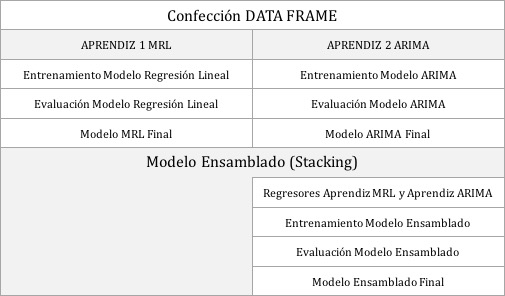
\includegraphics[width=5in]{ArquitecturaModeloEnsamblado}
    \caption{Proceso de Investigación para el Análisis del Modelo Predictivo (Fuente Propia)}
\end{figure}

Cada aprendiz es a su vez un modelo de aprendizaje automatizado con su propia metodología de investigación.

\subsubsection{Aprendiz 1: Modelo de Regresión Lineal}
\begin{itemize}
	\item El aprendiz 1 es un modelo de regresión lineal utilizando como variable dependiente el valor de la TRM para cada día del juego de datos y como regresores un arreglo asociado de cotizaciones del precio promedio mundial de los once productos principales de la canasta de exportación de Colombia entre los años 2010 y 2017.
	\item Para el juego de entrenamiento se selecciona un 70\% de los datos disponibles. Dicha selección se hace con la ayuda de la biblioteca CARET de R para funciones de aprendizaje automatizado.
	\item Para el juego de validación se selecciona un 30\% de los datos disponibles. Dicha selección también se hace con la ayuda de la biblioteca CARET de R para funciones de aprendizaje automatizado.
	\item La variable SEED se prefigura al valor arbitrario \emph{7556014} para propósitos de reproducibilidad de los datos.
	\item El aprendizaje automatizado no asegura que todos los regresores sean útiles o necesarios para una predicción dentro de los valores de confianza esperados. Existe la posibilidad que un número limitado de regresores cumpla con los mismos valores de predicción que la totalidad de los mismos y que el modelo generalice mejor al tener menos regresores (disminuyendo la inflación de la varianza como efecto secundario).
	\item Para determinar el número óptimo de regresores se procedió a armar el modelo de aprendizaje automatizado sumando un regresor a la vez y analizando los valores del coeficiente de determinación y coeficiente de correlación. Los valores finales del error mínimo cuadrático de cada modelo se comparan para determinar la mejor combinación de regresores.
	\item Como segunda validación para la combinación correcta de regresores, se utilizó el análisis \emph{Step\_AIC} (reducción óptima de regresores utilizando análisis combinatorio y el Criterio de Información de Aikake) con la biblioteca \emph{STEP\_AIC} de \emph{R}. El método \emph{STEP\_AIC} es intensivo en recursos de computación y no siempre arroja resultados superiores a los que un investigador pueda armar a mano utilizando técnicas visuales de exploración de datos.
\end{itemize}

\subsubsection{Aprendiz 2: Modelo ARIMA}
\begin{itemize}
	\item El aprendiz 2 es un modelo de pronostico ARIMA utilizando como serie de tiempo el valor de la TRM para cada día del juego de datos entre los años 2010 y 2017.
	\item Para el juego de entrenamiento se selecciona un 70\% de los datos disponibles. Dicha selección se hace con la ayuda de la biblioteca FORECAST de R para funciones de aprendizaje automatizado utilizando series de tiempo \cite{hyndman}.
	\item Para el juego de validación se selecciona un 30\% de los datos disponibles. Dicha selección también se hace con la ayuda de la biblioteca FORECAST de R para funciones de aprendizaje automatizado de series de tiempo.
	\item La variable SEED se prefigura al valor arbitrario \emph{7556014} para propósitos de reproducibilidad de los datos.
\end{itemize}

\subsubsection{Clasificador Ensamblado}
\begin{itemize}
	\item El clasificador ensamblado se toma como un arreglo de una variable dependiente (el valor de la TRM para cada día correspondiente al juego de datos) y dos variables independientes (los resultados de la predicción de los dos aprendices).
	\item Para el juego de entrenamiento se selecciona el 100\% de los datos disponibles. Dicha selección se hace con los resultados de las pruebas de evaluación de los dos aprendices iniciales \cite{popularEnsemble}.
	\item La variable SEED se prefigura al valor arbitrario \emph{7556014} para propósitos de reproducibilidad de los datos.
	\item El modelo se resuelve utilizando la metodología de Stacking como un modelo de regresión lineal \cite{smolyakov}.
\end{itemize}

\subsubsection{Validación del Modelo Ensamblado}
Se espera del modelo final un nivel de desempeño con predicciones dentro de un \(\alpha \leq 0.05\). Para tal fin dentro del diseño de investigación se valida el modelo sometiendo el mismo a un juego aleatorio de 100 datos de muestra que comprende:

\subsubsection{Esquema Visual del Modelo Predictivo}
El siguiente es el esquema visual del modelo predictivo donde se muestra como los resultados de los aprendices del modelo ARIMA y de regresión lineal múltiple se convierten en las entradas del modelo ensamblado.

\begin{figure}[H]
	\centering
	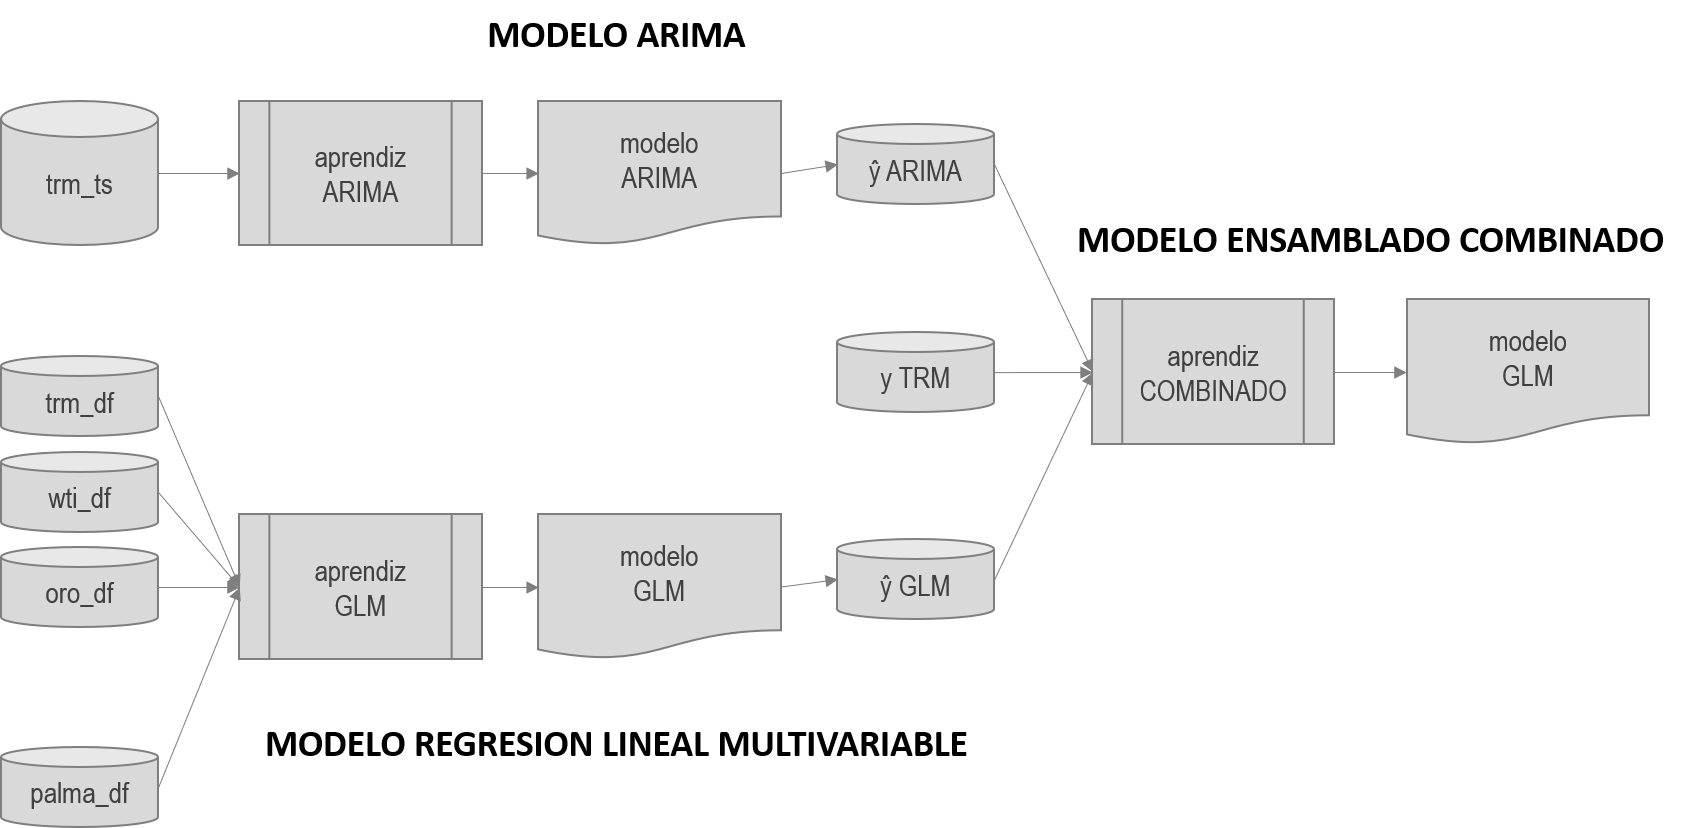
\includegraphics[width=5in]{images/EsquemaModeloPredictivo.png}	\caption{Esquema Modelo Predictivo}
\end{figure}

\begin{itemize}
	\item Resultados de predicción del modelo versus el modelo aprendiz 1 de regresión lineal multivariable.
	\item Resultados de predicción del modelo ensamblado versus el modelo aprendiz 2 ARIMA.
	\item Resultados de predicción del modelo ensamblado versus un intervalo de confianza del 99\%.
\end{itemize}

El modelo se considera óptimo para producción si pasa las tres pruebas de validación.

\section{Diseño de la Instrumentación}
El diseño de la instrumentación para el trabajo de laboratorio incluirá programas de software matemático para:

\begin{itemize}
    \item Recolectar las diferentes series de tiempo que servirán como variables dependientes (valor de la TRM) e independientes (regresores tales como las cotizaciones del barril de petróleo, quintal de café, etc.)
    \item Análisis exploratorio visual para determinar validez de los datos, muestras de autocorrelación y autocorrelación parcial a través de la prueba Dickey-Fueller
    \item Calce de la función de regresión lineal para las variables independientes
    \item Código para el modelo predictivo ensamblado
\end{itemize}

\subsection{Componentes de Investigación Series de Tiempo}
Un componente de aportación es cualquier rubro que se supone se exporta desde Colombia, aporta ingresos en dólares, y por lo tanto ayuda a equilibrar la balanza de pagos y demanda demanda de divisas - y por ende la TRM. Es importante hacer un análisis de cada uno de estos que debe incluir \cite{zumelMount}:

\begin{itemize}
	\item carga inicial como serie de tiempo (time series class)
	\item start(), end()
    \item summary()
    \item plot.ts()
    \item acf()
    \item pacf()
    \item descomponer en stl()
    \item prueba Dickey Fuller adf.test()
\end{itemize}

La carga inicial de datos para cualquier serie de tiempo se hace a través del servicio web de \textit{Quandl} (el siguiente ejemplo ilustrativo utiliza las cotizaciones del quintal de café).

\begin{lstlisting}[language=R]
# Load coffee prices as time series
library(Quandl)
library(tseries)

Quandl.api_key("KzzS8Vfxkw1ZgTWgU4jH")
coffee <- Quandl("ODA/PCOFFOTM_USD", collapse = "monthly", type = "ts")
head(coffee)
class(coffee)
cycle(coffee)
\end{lstlisting}

\subsection{EDA (Explorative Data Analysis)}
La forma más sencilla de ver los efectos del precio del café es revisar la tendencia del precio internacional y si ha habido efectos por temporada o alguna tendencia \cite{daroczi}.

\begin{lstlisting}[language=R]
plot.ts(coffee)
abline(reg = lm(coffee ~ time(coffee)))
\end{lstlisting}

\begin{figure}[H]
	\centering
	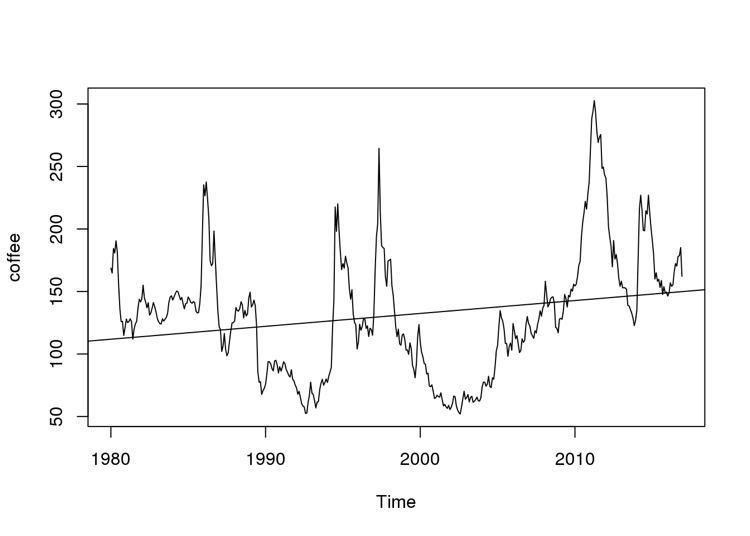
\includegraphics[width=5in]{correlacionTiempoCafe}
	\caption{Análisis EDA Cotización Internacional Café por quintal  (Fuente Propia)}
\end{figure}

Otro examen necesario es el de autocorrelación y autocorrelación parcial. Ambos análisis nos permiten ver si la serie es del tipo auto-regresiva o de promedios móviles \cite{hyndman}.

\begin{lstlisting}[language=R]
par(mfrow=c(1,2))
acf(coffee)
pacf(coffee)
\end{lstlisting}

\begin{figure}[H]
	\centering
	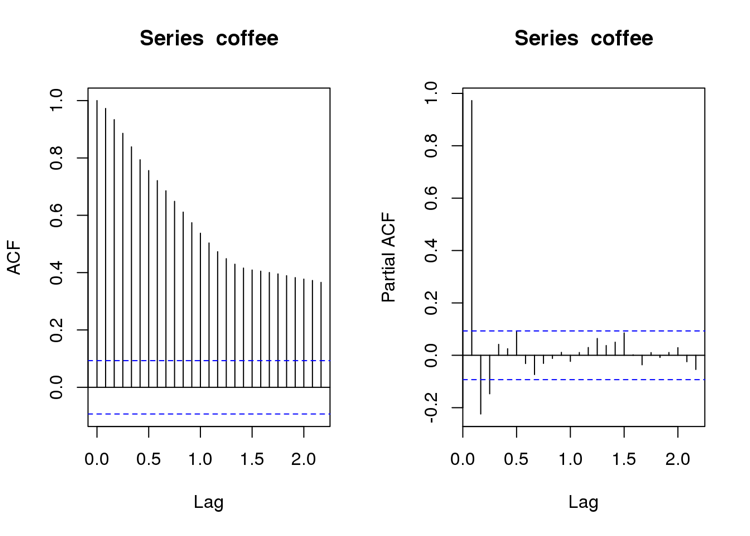
\includegraphics[width=5in]{autocorrelacion}\\
	\caption{Correlograma Precio Internacional del Café (Fuente Propia)}
\end{figure}

El último examen es la descomposición de la serie en datos, temporalidad y tendencia, para ver si alguno de estos elementos está presente.

\begin{lstlisting}[language=R]
decomp <- stl(coffee, s.window = 11)
plot(decomp)
\end{lstlisting}

\begin{figure}[H]
	\centering
	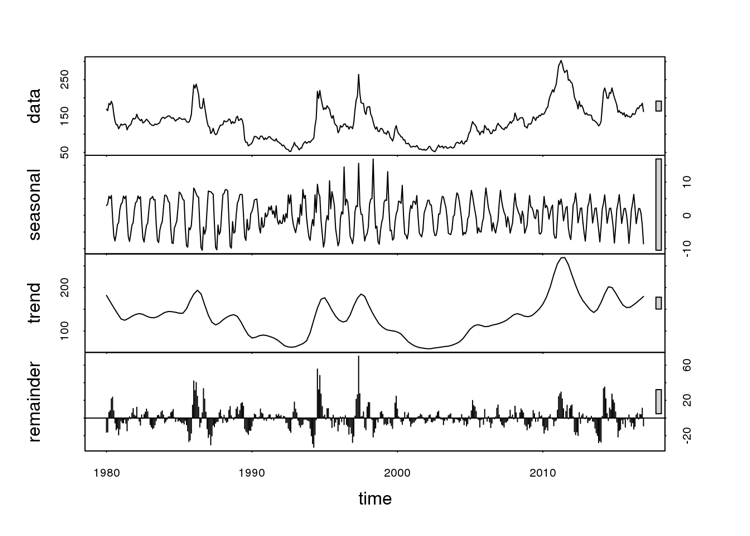
\includegraphics[width=5in]{decopSTLCafe}\\
	\caption{Descomposición STL Precio Internacional del Café (Fuente Propia)}
\end{figure}

El test \emph{Dickey Fuller} \cite{dickeyfuller} es la prueba mas importante para la verificación de la estacionalidad de una serie de tiempos. La literatura recomienda altamente someter todas las pruebas de series al test \emph{Dickey Fuller} antes de proceder con otros análisis \cite{hyndman}.

\begin{lstlisting}[language=R]
# Dickey Fuller Test for stationary time series
df <- adf.test(coffee, k = 12)
df$statistic
df$p.value
\end{lstlisting}

\subsection{Regresión Lineal con Calce de la Función de Predicción}
Los modelos de regresión lineal utilizan la biblioteca \emph{Quandl} para la extracción de datos y deben hacer la transformación del arreglo de datos a una serie de tiempos. Los datos serán colapsados de forma mensual y se revisará la fórmula de la función de calce para el coeficiente de correlación y determinación \cite{narayanachar}.

\begin{lstlisting}[language=R]
# Load oil prices as time series
library(Quandl)
library(tseries)

Quandl.api_key("KzzS8Vfxkw1ZgTWgU4jH")
wti <- Quandl("EIA/PET_RWTC_D", collapse = "monthly", type = "ts")
head(wti)
class(wti)
cycle(wti)

plot.ts(wti)
abline(reg = lm(wti ~ time(wti)), col="red")
fit = lm(wti ~ time(wti))
summary(fit)


Call:
lm(formula = wti ~ time(wti))

Residuals:
    Min      1Q  Median      3Q     Max
-45.031 -13.929  -0.368  11.399  80.925

Coefficients:
              Estimate Std. Error t value Pr(>|t|)
(Intercept) -4849.3862   213.2634  -22.74   <2e-16 ***
time(wti)       2.4439     0.1065   22.94   <2e-16 ***
---
Signif. codes:  0 '***' 0.001 '**' 0.01 '*' 0.05 '.' 0.1 ' ' 1

Residual standard error: 19.43 on 384 degrees of freedom
Multiple R-squared:  0.5782,	Adjusted R-squared:  0.5771
F-statistic: 526.4 on 1 and 384 DF,  p-value: < 2.2e-16
\end{lstlisting}

\begin{figure}[H]
	\centering
	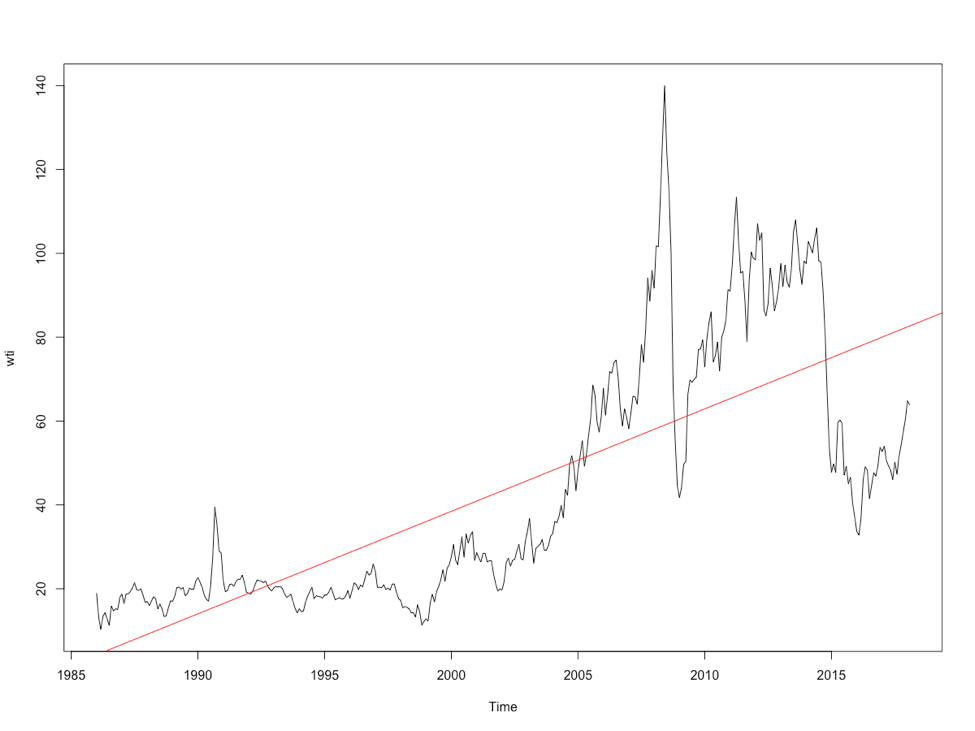
\includegraphics[width=5in]{regresionTiempoWTI}\\
	\caption{Descomposición STL Precio Internacional del Café (Fuente Propia)}
\end{figure}

\subsection{Modelo Predictivo Ensamblado}
El modelo predictivo ensamblado es el resultado del entrenamiento de un modelo predictivo de regresión lineal y un modelo ARIMA. Ambos modelos se combinan y se entrenan con la variable de valor real en común para ambos \cite{viswanathan}.

\begin{lstlisting}[language=R]
# Pseudo-codigo R simplificado
# Funcion de modelo ensamblado

# Cargar Data Frame con informacion de series de tiempo
library(caret)
set.seed(7556014)
data(featuresTRM)
data(TRM)
adData = data.frame(TRM, featuresTRM)
inTrain = createDataPartition(adData$TRM, p = 3/4)[[1]]
training = adData[ inTrain,]
testing = adData[-inTrain,]

set.seed(7556014)

modelo1 <- train(TRM ~ ., method = "glm", data = training)
modelo2 <- train(TRM ~ ., method = "ARIMA", data = training)

# Vectores de valores de prediccion de cada modelo
predVec1 <- predict(modelo1, testing)
predVec2 <- predict(modelo2, testing)

# Construccion de matriz de datos ensamblados (variable dependiente y predictor)
predDF <- data.frame(TRM = testing$TRM, predVec1, predVec2)

# Modelo combinado (fit)
combModelFit <- train(TRM ~ ., method = "glm", data = predDF)
finalPred <- predict(combModelFit, predDF)
\end{lstlisting}

\section{Diseño de muestreo}

Inicialmente, podemos calcular el tamaño de la muestra necesaria para nuestro estudio con la fórmula \cite{mendehall}:

\begin{equation}
   n =  (N* z^2*p*q)/(E^2*(N-1)+ z^2*p*q)
\end{equation}

El tamaño total de todas las cotizaciones de la TRM o del precio internacional del petróleo WTI es un número finito. Los mercados funcionan de lunes a viernes, por lo general las cincuenta y dos semanas del año. Para el uso común de la tasa de cambio, esta cifra se usa todos los días, por ejemplo cuando un consumidor usa una tarjeta de crédito y el banco debe referir al valor de la TRM aunque no sea día de operaciones bursátiles. Por lo que el número total de posibles cotizaciones oficiales en un año dado cualesquiera se determinan como:

\begin{equation}
    N_{regresor} = 365
\end{equation}

La fórmula es muy simple y equivale a sustituir cualquier variable regresor (por ejemplo, el valor del petróleo WTI) por los números reales de días del año.

\begin{equation}
    N_{wti} = 365
\end{equation}

Ende, existen 365 posibles valores de la cotización del petróleo WTI en un año cualesquiera. Dado que el modelo de predicción de aprendizaje automatizado utiliza datos del año 2010 al 2017 inclusive, podemos ampliar el universo dentro del período de estudio con la siguiente formula:
\begin{equation}
    n_{regresor} = 365 * 8 = 2920
\end{equation}

Nuestro universo por regresor equivale a dos mil novecientos veinte puntos de datos. Para un estudio con un nivel de confianza del 99\% y un error de estimación del 5\% calculamos el número de la muestra como una proporción, donde:

\begin{eqnarray*}
  N &=& 2,080 \text{ puntos de datos} \\
  p &=& 0.5 \\
  q &=& 0.5 \text{ o (1 – p)} \\
  z &=& 99\% \text{ o 2.575} \\
  e &=& 5\% \text{ o 0.05} \\
\end{eqnarray*}

Utilizamos el lenguaje R para resolver el cálculo:

\begin{lstlisting}[language=R]
N <- 2080
p <- 0.5
q <- 1 - p
z <- 2.575
E <- 0.05

muestra <- (N * z^2 * p * q) / ((N - 1) * E^2 + z^2 * p * q)
muestra
[1] 502.9681
\end{lstlisting}

El tamaño de la muestra es 503 puntos de datos por regresor a utilizar. Sin embargo, dado que los usos de técnicas de Ciencia de Datos nos permiten acceder a la biblioteca Quandl de forma de recolectar el universo entero de datos, utilizaremos los 2,920 puntos de datos para cada regresor, trabajando de esta forma con el universo entero y no la muestra. Este es un buen ejemplo del uso de Big Data \cite{pengMatsui} que no solo aplica a muestras grandes de universos extensos, sino al total de la data de un universo pequeño.

\subsubsection{Reglas de Imputación de Datos}
Es común que las bases de datos retornen series de datos incompletas para los días feriados o días sin cambio en la cotización del bien. Para determinar el valor de cualquier día incompleto, la investigación resolvió el método de imputación como la última cotización válida para el regresor.

\subsection{Observaciones Adicionales Sobre el Uso de Muestras dentro de Diseños de Investigación con Regresión Lineal}
No todos los autores están de acuerdo con el uso de la fórmula tradicional para el cálculo del número de muestras en un estudio de regresión lineal. William Dupont y Walton Plummer han discutido el uso de técnicas alternativas cuando los estudios (sobre todo los estudios clínicos) utilizan regresiones lineales multivariable \cite{dupontPlummer}. Dichas técnicas se apoyan en la identificación de diferentes pendientes en los análisis de regresión versus el uso de coeficientes (argumentando que es más fácil comparar visualmente pendientes versus coeficientes) y el manejo del poder estadístico $1 – \beta$. Sobre este último los autores manifiestan ajustar los niveles de poder para verificar en que momento del cambio se detecta diferencias de la pendiente de una hipótesis contra su hipótesis alternativa dentro de una muestra de n pacientes.

Al momento de preparar el diseño del estudio, las herramientas de medición y la muestra, el doctorando ha decidido no profundizar más en métodos menos tradicionales de cálculo de muestras en estudios de regresión lineal, dado que en el caso específico se utilizará la totalidad del universo, haciendo el cálculo de muestra innecesario.

\setcounter{chapter}{3}
\chapter{Resultados}
Contenidos por definir.

\chapter{Conclusiones y Recomendaciones}
La conclusión principal de la investigación doctoral es que los rubros de exportación de la economía Colombiana pueden ser utilizado como regresores de un modelo predictivo de la tasa de referencia del mercado. Cuando estos regresores se combinan con la serie de tiempo de la TRM misma a través del uso del aprendizaje automatizado, el resultado es un modelo ensamblado combinado parsimonioso y altamente preciso.

Cuando elevamos el nivel de análisis alrededor de los resultados del trabajo de laboratorio podemos ver conclusiones enfocadas en tres rubros:

\begin{enumerate}
  \item conclusiones específicas sobre el uso y validez de cada método de predicción utilizado en el aprendizaje automatizado como aprendiz
  \item conclusiones específicas sobre las ventajas de la metodología de métodos ensamblados
  \item conclusiones del uso de aprendizaje automatizado en la contabilidad de costos
\end{enumerate}

La Ciencia de Datos y el Aprendizaje Automatizado como disciplinas son áreas de la academia relativamente nuevas y con menor exposición en las universidades Latinoamericanas. El trabajo de investigación doctoral nos permite aportar recomendaciones al respecto de los siguientes temas:

\begin{itemize}
  \item recomendaciones sobre la implementación de una investigación de Ciencia de Datos utilizando Aprendizaje Automatizado
  \item recomendaciones sobre futuros trabajos de investigación resultantes de inquietudes que surgieron a lo largo del trabajo de laboratorio y a las cuales no se les pudo dar respuestas que satisfagan la curiosidad científica
\end{itemize}

\section{Conclusiones}
Cada método de aprendizaje automatizado utilizado en el siguiente trabajo de investigación tiene sus bondades. Para discutir cada uno con total objetividad, haremos referencia a una sola tabla comparativa de valores de desempeño y precisión.

\begin{table}[h!]
  \begin{center}
    \caption{Desempeño Comparativo de Métodos Machine Learning}
    \label{tab:table1}
    \begin{tabular}{c|c|c|c}
      \textbf{Indicador} & \textbf{ARIMA} & \textbf{Regresión Lineal} & \textbf{Modelo Ensamblado}\\
      \hline
      RMSE & 25.5473 &89.0524 & 24.8040 \\
      R2 & 0.9976 & 0.9714 & 0.9978 \\
    \end{tabular}
  \end{center}
\end{table}

\subsection{Modelo ARIMA}
El modelo ARIMA tuvo resultados por encima de las expectativas del investigador, con un valor de error cuadrático bajo y un valor de coeficiente de determinación alto, ciertamente superior al método de regresión lineal multivariable. La fortaleza del pronóstico ARIMA se fundamente en lo completo y robusto del juego de datos utilizado. La serie de tiempo de la TRM es estudiada por todo el sector contable, económico y financiero de Colombia, por lo que no fue sorpresa que de todas las series de datos está fuera la más accesible de estudio. El comportamiento de la serie de datos TRM también tienen una tendencia secular y de estacionalidad muy marcadas que se ajusta al uso de metodologías como ARIMA.

Dado el caso de no contar con otras metodologías o acceso a base de datos mayores para ampliar el rango de métodos potables, el uso de un aprendiz ARIMA puede solucionar el problema de pronosticar el valor futuro de la TRM sin necesidad de mayor complicación.

\subsection{Modelo de Regresión Lineal Multivariable}
El modelo de regresión lineal multivariable tuvo el desempeño menos preciso de los tres métodos estudiados. El valor del error cuadrático fue el mayor de los tres (aunque no necesariamente se puede decir que fue alto) y el coeficiente de determinación fue el menor de los tres (aunque fue alto estadísticamente hablando). El uso de los rubros de exportación como regresores se justifica con el calce ajustado del modelo, por lo que se considera un modelo robusto y parsimonioso. Sin embargo es un modelo más difícil de aplicar sin conocimientos de programación de métodos de aprendizaje automatizado y no rindió mejores pronósticos que el uso más sencillo de ARIMA.

\subsection{Modelo Ensamblado Stacking}
Correspondiendo con la literatura y los trabajos de autores como Daroczi, Leek, Peng y Tattar, el modelo ensamblado tuvo los mejores niveles de desempeño y precisión con el error cuadrático más bajo y el coeficiente de determinación más alto. La utilización de los dos métodos iniciales como entradas para un aprendiz ensamblado genera un método más robusto que se nutre de entradas pre-procesadas por los aprendices que las componen. Habiendo dicho esto, el desempeño obtenido por el método ensamblado no se puede considerar sino marginal en comparación con los aprendices que lo alimentan. La diferencia del error cuadrático es considerable si se mide contra el aprendiz de regresión lineal multivariable, pero poco notable contra el aprendiz ARIMA. De la misma forma, el valor del coeficiente de determinación su superior por menos de 0.026 contra el aprendiz de regresión lineal multivariable, pero nuevamente imperceptible versus el aprendiz ARIMA.

\subsection{Modelos de Aprendizaje Automatizado versus Modelos Ensamblados}
La utilización de la TRM en contratos de futuros o \emph{forwards} puede justificar la complejidad adicional de implementar un algoritmo compuesto. Para funciones de análisis de costos el overhead adicional de lidiar con un modelo ensamblado puede no hacer diferencias en el costeo final, sobre todo en cifras con redondeos a 2 decimales.

Para la organización moderna y de amplio alcance la complejidad adicional de la utilización de modelos ensamblados puede verse recompensada con el tiempo. El mayor nivel de precisión siempre redundará en mejores márgenes de utilidad y ganancias de productividad. En un ambiente dinámico y de bajo margen de utilidad como lo es el negocio de corretaje bursátil dicha precisión puede ser la diferencia entre la viabilidad de operación o no.

Para reportes ad-hoc, análisis de factibilidad, o toma rápida de decisiones, el uso de modelos ensamblados puede no ser la mejor respuesta. El trabajo de investigación doctoral llegó a un modelo parsimonioso y preciso con el uso del modelo ARIMA, el más sencillo de los tres de aplicar y entender. En el caso de tener que afrontar pronósticos de mediana exactitud, un modelo simple y rápido de aplicar puede satisfacer a la organización mejor que uno de mayor precisión pero intensivo en el uso de recursos y bases de datos extensas y validadas.

\section{Recomendaciones}
El trabajo de investigación arroja recomendaciones sobre la implementación de una investigación de Ciencia de Datos utilizando Aprendizaje Automatizado, y recomendaciones sobre futuros trabajos de investigación resultantes de inquietudes que surgieron a lo largo del trabajo de laboratorio.

\subsection{Implementación de Investigación de un Modelo Predictivo de Aprendizaje Automatizado}
Todas las fuentes de datos y todo el código fuente utilizado en el trabajo doctoral puede ubicarse en el sitio \emph{Github} del investigador. Ambos pueden ser utilizados bajo licencia MIT Open Source por cualquier estudiante, ejecutivo o persona que quiere conocer, ampliar, replicar, corroborar, mejorar y/o ampliar el conocimiento sobre la Ciencia de Datos y el Aprendizaje Automatizado.

Empero, utilizar el código provisto desde un computador personal es muy diferente a desplegar una investigación de Ciencia de Datos. Si para otros investigadores la recopilación de la información puede ser un problema crítico y el diseño de la instrumentación una decisión difícil para asegurar un análisis exitoso, el científico de datos se encuentra con problemas diferentes y típicos de su rama. La cantidad de datos disponible para cada investigación por lo general es exagerada y disponible con facilidad (razón por la cual se acuña el término BIG DATA). El problema pasa de la recolección al procesamiento de los datos. De igual manera el diseño de la instrumentación fue facilitado por la existencia de cientos de librerías disponibles en el lenguaje R. El investigador de datos pasa más tiempo decidiendo que juegos de datos son aplicables al

\setcounter{chapter}{5}
\chapter{Referencias}
Contenidos por definir.

\setcounter{chapter}{6}
\chapter{Otras Fuentes}
Contenidos por definir.

\setcounter{chapter}{7}
\chapter{Anexos}


\section{Bibliotecas de Programas}
La siguiente sección recopila los programas utilizados para el trabajo de investigación doctoral.

\subsection{Programa buildTRM.R}
El siguiente listado de secuencia de comandos R construye la serie de tiempos TRM para la tasa representativa del mercado.

\begin{lstlisting}[language=R]
# UBJ Doctorado en Administracion Gerencial
# Modelo Predictivo de la TRM Utilizando Machine Learning
# LIB ubj/code/buildTRM.R 
# FECHA 19/08/2018
# Ariel E. Meilij
#
# BRIEF Construye serie de datos TRM

library(Quandl)
library(tseries)
library(ggplot2)
library(ggfortify)
library(Hmisc)
library(corrplot)
library(PerformanceAnalytics)
library(reshape2)
library(ggpubr)

Quandl.api_key("KzzS8Vfxkw1ZgTWgU4jH")
trm_data <- Quandl("CURRFX/USDCOP")

# Limpiar serie de tiempo TRM en su data.frame
trm <- trm_data[, 1:2]
trm <- subset(trm, trm$Date > "2009-12-31")
trm <- subset(trm, trm$Rate > 1500)
colnames(trm) <- c("Date", "trm")

fechas <- seq(as.Date("2010-01-01"), as.Date("2017-12-31"), "days")
quote <- c(1:2922)
# Cargar como valor inicial valor mas antiguo de la serie de tiempo
last_quote <- trm[dim(trm)[1],2]

for(i in 1:2922)
{if(length(trm[which(trm$Date == fechas[i]), ]$trm))
{quote[i] <- trm[which(trm$Date == fechas[i]), ]$trm
last_quote <- trm[which(trm$Date == fechas[i]), ]$trm}
  else
  {quote[i] <- last_quote}
}

# Build into a time series
trm_ts <- ts(quote, start=c(2010,1,1), frequency=365)
plot(decompose(trm_ts))
save(trm_ts, file = "data/trm_ts")

# Build into data frame
trm_df <- data.frame(fechas, quote)
colnames(trm_df) = c("Date", "trm")
save(trm_df, file = "data/trm_df")
# EOC
\end{lstlisting}

\subsection{Programa buildBanana.R}
El siguiente listado de secuencia de comandos R construye la serie de tiempos banana con los valores de las cotizaciones mundiales de la tonelada de guineo.

\begin{lstlisting}[language=R]
# UBJ Doctorado en Administracion Gerencial
# Modelo Predictivo de la TRM Utilizando Machine Learning
# LIB ubj/code/buildBanana.R 
# FECHA 19/08/2018
# Ariel E. Meilij
#
# BRIEF Construye serie de datos del banano

library(Quandl)
library(tseries)
library(ggplot2)
library(ggfortify)
library(Hmisc)
library(corrplot)
library(PerformanceAnalytics)
library(reshape2)
library(ggpubr)

Quandl.api_key("KzzS8Vfxkw1ZgTWgU4jH")
banana_data <- Quandl("ODA/PBANSOP_USD")

# Limpiar serie de tiempo banana en su data.frame
banana <- subset(banana_data, banana_data$Date > "2009-12-31")
colnames(banana) <- c("Date", "banana")

fechas <- seq(as.Date("2010-01-01"), as.Date("2017-12-31"), "days")
quote <- c(1:2922)
# Cargar como valor inicial valor mas antiguo de la serie de tiempo
last_quote <- banana[dim(banana)[1],2]

for(i in 1:2922)
{if(length(banana[which(banana$Date == fechas[i]), ]$banana))
{quote[i] <- banana[which(banana$Date == fechas[i]), ]$banana
last_quote <- banana[which(banana$Date == fechas[i]), ]$banana}
  else
  {quote[i] <- last_quote}
}

# Build into a time series
banana_ts <- ts(quote, start=c(2010,1,1), end=c(2017,12,31), frequency=365)
plot(decompose(banana_ts))
save(banana_ts, file = "data/banana_ts")

# Build into data frame
banana_df <- data.frame(fechas, quote)
colnames(banana_df) = c("Date", "banana")
save(banana_df, file = "data/banana_df")
# EOC
\end{lstlisting}

\subsection{Programa buildCafe.R}
El siguiente listado de secuencia de comandos R construye la serie de tiempos café con los valores de las cotizaciones mundiales de la tonelada de café Arabiga.

\begin{lstlisting}[language=R]
# UBJ Doctorado en Administracion Gerencial
# Modelo Predictivo de la TRM Utilizando Machine Learning
# LIB ubj/code/buildCafe.R 
# FECHA 19/08/2018
# Ariel E. Meilij
#
# BRIEF Construye serie de datos cafe

library(Quandl)
library(tseries)
library(ggplot2)
library(ggfortify)
library(Hmisc)
library(corrplot)
library(PerformanceAnalytics)
library(reshape2)
library(ggpubr)

Quandl.api_key("KzzS8Vfxkw1ZgTWgU4jH")
cafe_data <- Quandl("CHRIS/ICE_KC1")

# Limpiar serie de tiempo cafe en su data.frame
cafe <- cafe_data[,c(1,5)]
cafe <- subset(cafe, cafe$Date > "2009-12-31")
cafe <- na.omit(cafe)
colnames(cafe) <- c("Date", "cafe")

fechas <- seq(as.Date("2010-01-01"), as.Date("2017-12-31"), "days")
quote <- c(1:2922)
# Cargar como valor inicial valor mas antiguo de la serie de tiempo
last_quote <- cafe[dim(cafe)[1],2]

for(i in 1:2922)
{if(length(cafe[which(cafe$Date == fechas[i]), ]$cafe))
{quote[i] <- cafe[which(cafe$Date == fechas[i]), ]$cafe
last_quote <- cafe[which(cafe$Date == fechas[i]), ]$cafe}
  else
  {quote[i] <- last_quote}
}

# Build into a time series
cafe_ts <- ts(quote, start=c(2010,1,1), end=c(2017,12,31), frequency=365)
plot(decompose(cafe_ts))
save(cafe_ts, file = "data/cafe_ts")

# Build into data frame
cafe_df <- data.frame(fechas, quote)
colnames(cafe_df) = c("Date", "cafe")
save(cafe_df, file = "data/cafe_df")
# EOC
\end{lstlisting}

\subsection{Programa buildCarbon.R}
El siguiente listado construye la serie de tiempos carbón con los precios de las cotizaciones mundiales de la tonelada de carbón.

\begin{lstlisting}[language=R]
# UBJ Doctorado en Administracion Gerencial
# Modelo Predictivo de la TRM Utilizando Machine Learning
# LIB ubj/code/buildCarbon.R 
# FECHA 19/08/2018
# Ariel E. Meilij
#
# BRIEF Construye serie de datos carbon

library(Quandl)
library(tseries)
library(ggplot2)
library(ggfortify)
library(Hmisc)
library(corrplot)
library(PerformanceAnalytics)
library(reshape2)
library(ggpubr)

Quandl.api_key("KzzS8Vfxkw1ZgTWgU4jH")
carbon_data <- Quandl("EIA/COAL")

# Limpiar serie de tiempo CARBON en su data.frame
carbon <- carbon_data[, 1:2]
carbon <- subset(carbon, carbon$`Week Ended` > "2009-12-31")
colnames(carbon) <- c("Date", "carbon")

fechas <- seq(as.Date("2010-01-01"), as.Date("2017-12-31"), "days")
quote <- c(1:2922)
# Cargar como valor inicial valor mas antiguo de la serie de tiempo
last_quote <- carbon[dim(carbon)[1],2]

for(i in 1:2922)
{if(length(carbon[which(carbon$Date == fechas[i]), ]$carbon))
{quote[i] <- carbon[which(carbon$Date == fechas[i]), ]$carbon
last_quote <- carbon[which(carbon$Date == fechas[i]), ]$carbon}
  else
  {quote[i] <- last_quote}
}

# Build into a time series
carbon_ts <- ts(quote, start=c(2010,1,1), end=c(2017,12,31), frequency=365)
plot(decompose(carbon_ts))
save(carbon_ts, file = "data/carbon_ts")

# Build into data frame
carbon_df <- data.frame(fechas, quote)
colnames(carbon_df) = c("Date", "carbon")
save(carbon_df, file = "data/carbon_df")
# EOC
\end{lstlisting}

\subsection{Programa buildGasoil.R}
El siguiente programa construye la serie de tiempo gasoil con los precios internacionales del gasoil en galones.

\begin{lstlisting}[language=R]
# UBJ Doctorado en Administracion Gerencial
# Modelo Predictivo de la TRM Utilizando Machine Learning
# LIB ubj/code/buildgasoil.R 
# FECHA 19/08/2018
# Ariel E. Meilij
#
# BRIEF Construye serie de datos del banano

library(Quandl)
library(tseries)
library(ggplot2)
library(ggfortify)
library(Hmisc)
library(corrplot)
library(PerformanceAnalytics)
library(reshape2)
library(ggpubr)

Quandl.api_key("KzzS8Vfxkw1ZgTWgU4jH")
gasoil_data <- Quandl("NASDAQOMX/NQCIGOER")

# Limpiar serie de tiempo gasoil en su data.frame
gasoil <- gasoil_data[, c(1:2)]
gasoil <- subset(gasoil, gasoil$`Trade Date` > "2009-12-31")
gasoil <- subset(gasoil, gasoil$`Index Value` > 0)
colnames(gasoil) <- c("Date", "gasoil")

fechas <- seq(as.Date("2010-01-01"), as.Date("2017-12-31"), "days")
quote <- c(1:2922)
# Cargar como valor inicial valor mas antiguo de la serie de tiempo
last_quote <- gasoil[dim(gasoil)[1],2]

for(i in 1:2922)
{if(length(gasoil[which(gasoil$Date == fechas[i]), ]$gasoil))
{quote[i] <- gasoil[which(gasoil$Date == fechas[i]), ]$gasoil
last_quote <- gasoil[which(gasoil$Date == fechas[i]), ]$gasoil}
  else
  {quote[i] <- last_quote}
}

# Build into a time series
gasoil_ts <- ts(quote, start=c(2010,1,1), end=c(2017,12,31), frequency=365)
plot(decompose(gasoil_ts))
save(gasoil_ts, file = "data/gasoil_ts")

# Build into data frame
gasoil_df <- data.frame(fechas, quote)
colnames(gasoil_df) = c("Date", "gasoil")
save(gasoil_df, file = "data/gasoil_df")
# EOC
\end{lstlisting}

\subsection{Programa buildHulla.R}
El siguiente programa construye la serie de tiempo hulla con las cotizaciones mundiales de la tonelada métrica de hulla térmica. 

\begin{lstlisting}[language=R]
# UBJ Doctorado en Administracion Gerencial
# Modelo Predictivo de la TRM Utilizando Machine Learning
# LIB ubj/code/buildHulla.R 
# FECHA 19/08/2018
# Ariel E. Meilij
#
# BRIEF Construye serie de datos hulla termica

library(Quandl)
library(tseries)
library(ggplot2)
library(ggfortify)
library(Hmisc)
library(corrplot)
library(PerformanceAnalytics)
library(reshape2)
library(ggpubr)

Quandl.api_key("KzzS8Vfxkw1ZgTWgU4jH")
hulla_data <- Quandl("CHRIS/SGX_CFF3")

# Limpiar serie de tiempo HULLA en su data.frame
hulla <- hulla_data[, c(1,6)]
hulla <- subset(hulla, hulla$Date > "2009-12-31")
colnames(hulla) <- c("Date", "hulla")

fechas <- seq(as.Date("2010-01-01"), as.Date("2017-12-31"), "days")
quote <- c(1:2922)
# Cargar como valor inicial valor mas antiguo de la serie de tiempo
last_quote <- hulla[dim(hulla)[1],2]

for(i in 1:2922)
{if(length(hulla[which(hulla$Date == fechas[i]), ]$hulla))
{quote[i] <- hulla[which(hulla$Date == fechas[i]), ]$hulla
last_quote <- hulla[which(hulla$Date == fechas[i]), ]$hulla}
  else
  {quote[i] <- last_quote}
}

# Build into a time series
hulla_ts <- ts(quote, start=c(2010,1,1), end=c(2017,12,31), frequency=365)
plot(decompose(hulla_ts))
save(hulla_ts, file = "data/hulla_ts")

# Build into data frame
hulla_df <- data.frame(fechas, quote)
colnames(hulla_df) = c("Date", "hulla")
save(hulla_df, file = "data/hulla_df")
# EOC
\end{lstlisting}

\subsection{Programa buildNiquel.R}
El siguiente programa construye la serie de tiempo níquel con las cotizaciones mundiales de la tonelada métrica de ferroníquel.

\begin{lstlisting}[language=R]
# UBJ Doctorado en Administracion Gerencial
# Modelo Predictivo de la TRM Utilizando Machine Learning
# LIB ubj/code/buildNiquel.R 
# FECHA 19/08/2018
# Ariel E. Meilij
#
# BRIEF Construye serie de datos del niquel

library(Quandl)
library(tseries)
library(ggplot2)
library(ggfortify)
library(Hmisc)
library(corrplot)
library(PerformanceAnalytics)
library(reshape2)
library(ggpubr)

Quandl.api_key("KzzS8Vfxkw1ZgTWgU4jH")
niquel_data <- Quandl("ODA/PNICK_USD")
# niquel_data <- Quandl("LME/PR_NI") FUENTE ALTERNA PERO INCOMPLETA

# Limpiar serie de tiempo niquel en su data.frame
# niquel_data <- niquel_data[, c(1,2)]
niquel <- subset(niquel_data, niquel_data$Date > "2009-12-31")
#niquel <- na.omit(niquel)
colnames(niquel) <- c("Date", "niquel")

fechas <- seq(as.Date("2010-01-01"), as.Date("2017-12-31"), "days")
quote <- c(1:2922)
# Cargar como valor inicial valor mas antiguo de la serie de tiempo
last_quote <- niquel[dim(niquel)[1],2]

for(i in 1:2922)
{if(length(niquel[which(niquel$Date == fechas[i]), ]$niquel))
{quote[i] <- niquel[which(niquel$Date == fechas[i]), ]$niquel
last_quote <- niquel[which(niquel$Date == fechas[i]), ]$niquel}
  else
  {quote[i] <- last_quote}
}

# Build into a time series
niquel_ts <- ts(quote, start=c(2010,1,1), end=c(2017,12,31), frequency=365)
plot(decompose(niquel_ts))
save(niquel_ts, file = "data/niquel_ts")

# Build into data frame
niquel_df <- data.frame(fechas, quote)
colnames(niquel_df) = c("Date", "niquel")
save(niquel_df, file = "data/niquel_df")
# EOC
\end{lstlisting}

\subsection{Programa buildOro.R}
El siguiente programa construye la serie de tiempo oro con los precios de cotización de la onza de oro Troy.

\begin{lstlisting}[language=R]
# UBJ Doctorado en Administracion Gerencial
# Modelo Predictivo de la TRM Utilizando Machine Learning
# LIB ubj/code/buildOro.R 
# FECHA 19/08/2018
# Ariel E. Meilij
#
# BRIEF Construye serie de datos oro

library(Quandl)
library(tseries)
library(ggplot2)
library(ggfortify)
library(Hmisc)
library(corrplot)
library(PerformanceAnalytics)
library(reshape2)
library(ggpubr)

Quandl.api_key("KzzS8Vfxkw1ZgTWgU4jH")
gold_data <- Quandl("WGC/GOLD_DAILY_USD")

# Limpiar serie de tiempo GOLD en su data.frame
oro <- subset(gold_data, gold_data$Date > "2009-12-31")
colnames(oro) <- c("Date", "oro")

fechas <- seq(as.Date("2010-01-01"), as.Date("2017-12-31"), "days")
quote <- c(1:2922)
# Cargar como valor inicial valor mas antiguo de la serie de tiempo
last_quote <- oro[dim(oro)[1],2]

for(i in 1:2922)
{if(length(oro[which(oro$Date == fechas[i]), ]$oro))
{quote[i] <- oro[which(oro$Date == fechas[i]), ]$oro
last_quote <- oro[which(oro$Date == fechas[i]), ]$oro}
  else
  {quote[i] <- last_quote}
}

# Build into a time series
oro_ts <- ts(quote, start=c(2010,1,1), end=c(2017,12,31), frequency=365)
plot(decompose(oro_ts))
save(oro_ts, file = "data/oro_ts")

# Build into data frame
oro_df <- data.frame(fechas, quote)
colnames(oro_df) = c("Date", "oro")
save(oro_df, file = "data/oro_df")
# EOC
\end{lstlisting}

\subsection{Programa buildPalma.R}
El siguiente programa construye la serie de tiempo palma, con las cotizaciones mundiales del galón de aceite de palma.

\begin{lstlisting}[language=R]
# buildPalma.R
# 2018-08-15
# Ariel E. Meilij
# UBJ - DBA

# Build palm oil time series and expand
# 2010-01-01 thru 2017-12-31
# Fill-in NA's or 0 values
# Last known quote takes precedence

library(Quandl)
library(tseries)
library(ggplot2)
library(ggfortify)
library(Hmisc)
library(corrplot)
library(PerformanceAnalytics)
library(reshape2)
library(ggpubr)

Quandl.api_key("KzzS8Vfxkw1ZgTWgU4jH")
palma_data <- Quandl("ODA/PPOIL_USD")

palma <- subset(palma_data, palma_data$Date > "2009-12-01")
colnames(palma) <- c("Date", "palma")

fechas <- seq(as.Date("2010-01-01"), as.Date("2017-12-31"), "days")
quote <- c(1:2922)
last_quote <- palma[dim(palma)[1],2]

for(i in 1:2922)
{if(length(palma[which(palma$Date == fechas[i]), ]$palma))
  {quote[i] <- palma[which(palma$Date == fechas[i]), ]$palma
  last_quote <- palma[which(palma$Date == fechas[i]), ]$palma}
      else
  {quote[i] <- last_quote}
}

qplot(x = fechas, y = quote, geom = "line", main = "Cotizacion Aceite de Palma (2010-2017)")

# Build into a time series
palma_ts <- ts(quote, start=c(2010,1,1), end=c(2017,12,31), frequency=365)
plot(decompose(palma_ts))
save(palma_ts, file = "data/palma_ts")

# Build into data frame
palma_df <- data.frame(fechas, quote)
colnames(palma_df) = c("Date", "palma")
save(palma_df, file = "data/palma_df")

# EOC
\end{lstlisting}

\subsection{Programa buildPolipropileno.R}
El siguiente programa construye la serie polipropileno con las cotizaciones mundiales de la tonelada métrica de polipropileno.

\begin{lstlisting}[language=R]
# UBJ Doctorado en Administracion Gerencial
# Modelo Predictivo de la TRM Utilizando Machine Learning
# LIB ubj/code/buildPolipropileno.R 
# FECHA 19/08/2018
# Ariel E. Meilij
#
# BRIEF Construye serie de datos prolipropileno

library(Quandl)
library(tseries)
library(ggplot2)
library(ggfortify)
library(Hmisc)
library(corrplot)
library(PerformanceAnalytics)
library(reshape2)
library(ggpubr)

Quandl.api_key("KzzS8Vfxkw1ZgTWgU4jH")
polipropileno_data <- Quandl("FRED/WPU091303223")

# Limpiar serie de tiempo polipropileno en su data.frame
polipropileno <- subset(polipropileno_data, polipropileno_data$Date > "2009-12-31")
colnames(polipropileno) <- c("Date", "polipropileno")

fechas <- seq(as.Date("2010-01-01"), as.Date("2017-12-31"), "days")
quote <- c(1:2922)
# Cargar como valor inicial valor mas antiguo de la serie de tiempo
last_quote <- polipropileno[dim(polipropileno)[1],2]

for(i in 1:2922)
{if(length(polipropileno[which(polipropileno$Date == fechas[i]), ]$polipropileno))
{quote[i] <- polipropileno[which(polipropileno$Date == fechas[i]), ]$polipropileno
last_quote <- polipropileno[which(polipropileno$Date == fechas[i]), ]$polipropileno}
  else
  {quote[i] <- last_quote}
}

# Build into a time series
polipropileno_ts <- ts(quote, start=c(2010,1,1), end=c(2017,12,31), frequency=365)
plot(decompose(polipropileno_ts))
save(polipropileno_ts, file = "data/polipropileno_ts")

# Build into data frame
polipropileno_df <- data.frame(fechas, quote)
colnames(polipropileno_df) = c("Date", "polipropileno")
save(polipropileno_df, file = "data/polipropileno_df")
# EOC
\end{lstlisting}

\subsection{Programa buildWti.R}
El siguiente programa construye la serie de tiempo wti, que es el resultante de las cotizaciones mundiales del barril de petróleo tipo West Texas. 
\begin{lstlisting}[language=R]
# UBJ Doctorado en Administracion Gerencial
# Modelo Predictivo de la TRM Utilizando Machine Learning
# LIB ubj/code/buildWti.R 
# FECHA 19/08/2018
# Ariel E. Meilij
#
# BRIEF Construye serie de datos petroleo WTI

library(Quandl)
library(tseries)
library(ggplot2)
library(ggfortify)
library(Hmisc)
library(corrplot)
library(PerformanceAnalytics)
library(reshape2)
library(ggpubr)

Quandl.api_key("KzzS8Vfxkw1ZgTWgU4jH")
wti_data <- Quandl("EIA/PET_RWTC_D")

# Limpiar serie de tiempo wti en su data.frame
wti <- subset(wti_data, wti_data$Date > "2009-12-31")
colnames(wti) <- c("Date", "wti")

fechas <- seq(as.Date("2010-01-01"), as.Date("2017-12-31"), "days")
quote <- c(1:2922)
# Cargar como valor inicial valor mas antiguo de la serie de tiempo
last_quote <- wti[dim(wti)[1],2]

for(i in 1:2922)
{if(length(wti[which(wti$Date == fechas[i]), ]$wti))
{quote[i] <- wti[which(wti$Date == fechas[i]), ]$wti
last_quote <- wti[which(wti$Date == fechas[i]), ]$wti}
  else
  {quote[i] <- last_quote}
}

# Build into a time series
wti_ts <- ts(quote, start=c(2010,1,1), end=c(2017,12,31), frequency=365)
plot(decompose(wti_ts))
save(wti_ts, file = "data/wti_ts")

# Build into data frame
wti_df <- data.frame(fechas, quote)
colnames(wti_df) = c("Date", "wti")
save(wti_df, file = "data/wti_df")
# EOC
\end{lstlisting}

\subsection{visualRegresoresTS.R}
El siguiente programa utiliza un gráfico compuesto para aplicar técnicas \emph{EDA} de análisis visual y verificar la integridad de las series de tiempo antes de aplicar los algoritmos de aprendizaje automatizado.

\begin{lstlisting}[language=R]
# UBJ Doctorado en Administracion Gerencial
# Modelo Predictivo de la TRM Utilizando Machine Learning
# LIB ubj/code/visualRegresoresTS 
# FECHA 19/08/2018
# Ariel E. Meilij
#
# BRIEF EDA regresores TRM en forma de serie de tiempo

# Carga de librerias necesarias
library(tseries)
library(ggplot2)
library(ggfortify)
library(Hmisc)
library(corrplot)
library(PerformanceAnalytics)
library(reshape2)
library(ggpubr)

# Cargar data frames en memoria
load("data/trm_df")
load("data/palma_df")
load("data/oro_df")
load("data/wti_df")
load("data/cafe_df")
load("data/banana_df")
load("data/niquel_df")
load("data/gasoil_df")
load("data/polipropileno_df")
load("data/hulla_df")
load("data/carbon_df")

# Multiple Graph
graf1 <- ggplot(trm_df, aes(x = Date, y = trm)) + geom_line(color = "#00AFBB", size = 1) + 
  xlab("Fechas") + ylab("Cotizacion TRM")
graf2 <- ggplot(palma_df, aes(x = Date, y = palma)) + geom_line(color = "#00AFBB", size = 1) + 
  xlab("Fechas") + ylab("Cotizacion Aceite de Palma")
graf3 <- ggplot(oro_df, aes(x = Date, y = oro)) + geom_line(color = "#00AFBB", size = 1) + 
  xlab("Fechas") + ylab("Cotizacion Oro")
graf4 <- ggplot(wti_df, aes(x = Date, y = wti)) + geom_line(color = "#00AFBB", size = 1) + 
  xlab("Fechas") + ylab("Cotizacion Petroleo WTI")
graf5 <- ggplot(cafe_df, aes(x = Date, y = cafe)) + geom_line(color = "#00AFBB", size = 1) + 
  xlab("Fechas") + ylab("Cotizacion Cafe")
graf6 <- ggplot(banana_df, aes(x = Date, y = banana)) + geom_line(color = "#00AFBB", size = 1) + 
  xlab("Fechas") + ylab("Cotizacion Banano")
graf7 <- ggplot(niquel_df, aes(x = Date, y = niquel)) + geom_line(color = "#00AFBB", size = 1) + 
  xlab("Fechas") + ylab("Cotizacion Ferroniquel")
graf8 <- ggplot(gasoil_df, aes(x = Date, y = gasoil)) + geom_line(color = "#00AFBB", size = 1) + 
  xlab("Fechas") + ylab("Cotizacion Gasoil")
graf9 <- ggplot(polipropileno_df, aes(x = Date, y = polipropileno)) + geom_line(color = "#00AFBB", size = 1) + 
  xlab("Fechas") + ylab("Cotizacion Polipropileno")
graf10 <- ggplot(hulla_df, aes(x = Date, y = hulla)) + geom_line(color = "#00AFBB", size = 1) + 
  xlab("Fechas") + ylab("Cotizacion Hulla Termica")
graf11 <- ggplot(carbon_df, aes(x = Date, y = carbon)) + geom_line(color = "#00AFBB", size = 1) + 
  xlab("Fechas") + ylab("Cotizacion Carbon")

ggarrange(graf1, graf2, graf3, graf4, graf5, graf6, graf7, graf8, graf9, graf10, graf11 + rremove("x.text"), 
          labels = c("TRM", "PALMA", "ORO", "WTI", "CAFE", "BANANA", "FERRONIQUEL", "GASOIL", "POLIPROPILENO", "HULLA TERMICA", "CARBON" ),
          ncol = 3, nrow = 4)
\end{lstlisting}

\subsection{Programa testMLRegression.R}
El siguiente programa fue utilizado como punto intermedio en el trabajo de laboratorio para evaluar el potencial de un modelo de regresión lineal y los regresores candidatos. El mismo no utiliza aprendizaje automatizado sino que aplica un modelo tradicional de regresión lineal multivariable.

\begin{lstlisting}[language=R]
# UBJ Doctorado en Administracion Gerencial
# Modelo Predictivo de la TRM Utilizando Machine Learning
# LIB ubj/code/testMLRegression
# FECHA 19/08/2018
# Ariel E. Meilij
#
# BRIEF Evalua Modelo de Regresion Multivariable con Machine Learning
# Utiliza biblioteca CARET para aprendizaje automatizado

# Carga de librerias necesarias
library(tseries)
library(ggplot2)
library(ggfortify)
library(Hmisc)
library(corrplot)
library(PerformanceAnalytics)
library(reshape2)
library(ggpubr)
library(caret)

# Cargar data frames en memoria
load("data/trm_df")
load("data/palma_df")
load("data/oro_df")
load("data/wti_df")
load("data/cafe_df")
load("data/banana_df")
load("data/niquel_df")
load("data/gasoil_df")
load("data/polipropileno_df")
load("data/hulla_df")
load("data/carbon_df")

# Merge data frames
df1 <- merge(trm_df, palma_df)
df1 <- merge(df1, oro_df)
df1 <- merge(df1, wti_df)
df1 <- merge(df1, cafe_df)
df1 <- merge(df1, banana_df)
df1 <- merge(df1, niquel_df)
df1 <- merge(df1, gasoil_df)
df1 <- merge(df1, polipropileno_df)
df1 <- merge(df1, hulla_df)
df1 <- merge(df1, carbon_df)
summary(df1)

# Eliminar datos, no hacen falta para este ejercicio
df_data <- df1[, 2:12]
rm(df1, trm_df, palma_df, oro_df, wti_df, cafe_df, banana_df, niquel_df, gasoil_df, polipropileno_df, hulla_df, carbon_df)

# Crear juegos de datos para entrenamiento y prueba
set.seed(7556014)
inTrain <- createDataPartition(y = df_data$trm, p = 0.7, list = FALSE)
training <- df_data[inTrain, ]
testing <- df_data[-inTrain, ]

# Comenzar entrenamiento
modelFit <- train(trm ~ ., data = training, method = "glm")

# Graficas de verificacion de modelo
plot(modelFit$finalModel)
plot(modelFit$finalModel, 4, pch = 19, cex = 0.5, col = "#00000010")
plot(modelFit$finalModel$residuals, pch = 19)
abline(0,0, col = "red")

# Plot Data Entrenada en Prediccion vs. Valores Reales
valores_reales <- df_data[inTrain, 1]
valores_prediccion <- predict(modelFit, training[,2:11])
testVector <- data.frame(valores_prediccion, valores_reales)
ggplot(aes(x = valores_prediccion, y = valores_reales), data = testVector) + 
  geom_point(alpha = 0.05)  + geom_smooth(method='lm',formula=y~x, colour = "green") + 
  labs(x = "Valores Prediccion", y = "Valores Reales", 
       title = "Valores Reales vs. Valores Prediccion Modelo Entrenado Regresion Multivariable")

# Plot Data de Prueba vs. Valores Reales
valores_reales <- df_data[-inTrain, 1]
valores_prediccion <- predict(modelFit, testing[,2:11])
testVector <- data.frame(valores_prediccion, valores_reales)
ggplot(aes(x = valores_prediccion, y = valores_reales), data = testVector) + 
  geom_point(alpha = 0.05)  + geom_smooth(method='lm',formula=y~x, colour = "yellow") +
  labs(x = "Valores Prediccion", y = "Valores Reales", 
       title = "Valores Reales vs. Valores Prediccion Data Validacion Regresion Multivariable")

# Test individual de valores aleatorios comparativos
indices_aleatorios <-  sample.int(dim(inTrain)[1], 20)
y_values <- df_data[indices_aleatorios, 1]
y_hat <- predict(modelFit, df_data[indices_aleatorios, 2:11])
testMatrix <- data.frame(y_values, y_hat, round(((y_hat/y_values)-1)*100,1))
colnames(testMatrix) = c("VALOR REAL", "PREDICCION", "ERROR %")
print(testMatrix)
print(mean(testMatrix$`ERROR %`))

# Grafica Residuales
residuales <- modelFit$finalModel$residuals
indice <- seq(1:2047)
data_residuales <- data.frame(residuales, indice)
ggplot(aes(y = residuales, x = indice), data = data_residuales) + geom_jitter(alpha = 1/05) +
  labs(y = "Error Aleatorio", x = "", title = "Valores Residuales")
\end{lstlisting}

\subsection{Programa testAutoARIMA.R}
El siguiente programa construye el modelo de pronostico ARIMA utilizando la biblioteca de aprendizaje automatizado \emph{forecast}.

\begin{lstlisting}[language=R]
# UBJ Doctorado en Administracion Gerencial
# Modelo Predictivo de la TRM Utilizando Machine Learning
# LIB ubj/code/testAutoARIMA 
# FECHA 19/08/2018
# Ariel E. Meilij
#
# BRIEF Pronostico de la TRM utilizando machine learning con ARIMA

library(forecast)
library(ggplot2)

load("data/trm_ts")

# Descomposicion de serie de tiempo TRM
plot(decompose(trm_ts))

# Evaluar autocorrelacion
par(mfrow=c(1,2))
acf(trm_ts)
pacf(trm_ts)

# Utilizar funcion auto.arima para modelo automatico ARIMA
modelFit <- auto.arima(trm_ts)

# Plot Data de Prueba vs. Valores Reales
valores_reales <- trm_ts
valores_prediccion <- modelFit$fitted
testVector <- data.frame(valores_prediccion, valores_reales)
ggplot(aes(x = valores_prediccion, y = valores_reales), data = testVector) + 
  geom_point(alpha = 0.05) + 
  geom_smooth(method='lm',formula=y~x, colour = "gray") +
  labs(x = "Valores Prediccion", y = "Valores Reales", 
       title = "Valores Reales vs. Valores Prediccion ARIMA(3,1,2) para TRM 2010-2017 ")

# Test individual de valores aleatorios comparativos
indices_aleatorios <-  sample.int(length(trm_ts), 100)
y_values <- trm_ts[indices_aleatorios]
y_hat <- modelFit$fitted[indices_aleatorios]
testMatrix <- data.frame(y_values, y_hat, round(((y_hat/y_values)-1)*100,1))
colnames(testMatrix) = c("VALOR REAL", "PREDICCION", "ERROR %")
print(testMatrix)
print(mean(testMatrix$`ERROR %`))

# Plot del Test
qplot(y = y_values, x = y_hat, data = testMatrix, show.legend = TRUE,
      main = "Test Aleatorio Valores Reales vs. Prediccion") + geom_smooth(formula = y~x) 
\end{lstlisting}

\subsection{Programa testMLRegression.R}
El siguiente programa utiliza la biblioteca \emph{CARET} para crear un modelo de regresión multivariable con aprendizaje automatizado.

\begin{lstlisting}[language=R]
# UBJ Doctorado en Administracion Gerencial
# Modelo Predictivo de la TRM Utilizando Machine Learning
# LIB ubj/code/testMLRegression
# FECHA 19/08/2018
# Ariel E. Meilij
#
# BRIEF Evalua Modelo de Regresion Multivariable con Machine Learning
# Utiliza biblioteca CARET para aprendizaje automatizado

# Carga de librerias necesarias
library(tseries)
library(ggplot2)
library(ggfortify)
library(Hmisc)
library(corrplot)
library(PerformanceAnalytics)
library(reshape2)
library(ggpubr)
library(caret)

# Cargar data frames en memoria
load("data/trm_df")
load("data/palma_df")
load("data/oro_df")
load("data/wti_df")
load("data/cafe_df")
load("data/banana_df")
load("data/niquel_df")
load("data/gasoil_df")
load("data/polipropileno_df")
load("data/hulla_df")
load("data/carbon_df")

# Merge data frames
df1 <- merge(trm_df, palma_df)
df1 <- merge(df1, oro_df)
df1 <- merge(df1, wti_df)
df1 <- merge(df1, cafe_df)
df1 <- merge(df1, banana_df)
df1 <- merge(df1, niquel_df)
df1 <- merge(df1, gasoil_df)
df1 <- merge(df1, polipropileno_df)
df1 <- merge(df1, hulla_df)
df1 <- merge(df1, carbon_df)
summary(df1)

# Eliminar datos, no hacen falta para este ejercicio
df_data <- df1[, 2:12]
rm(df1, trm_df, palma_df, oro_df, wti_df, cafe_df, banana_df, niquel_df, gasoil_df, polipropileno_df, hulla_df, carbon_df)

# Crear juegos de datos para entrenamiento y prueba
set.seed(7556014)
inTrain <- createDataPartition(y = df_data$trm, p = 0.7, list = FALSE)
training <- df_data[inTrain, ]
testing <- df_data[-inTrain, ]

# Comenzar entrenamiento
modelFit <- train(trm ~ ., data = training, method = "glm")

# Graficas de verificacion de modelo
plot(modelFit$finalModel)
plot(modelFit$finalModel, 4, pch = 19, cex = 0.5, col = "#00000010")
plot(modelFit$finalModel$residuals, pch = 19)
abline(0,0, col = "red")

# Plot Data Entrenada en Prediccion vs. Valores Reales
valores_reales <- df_data[inTrain, 1]
valores_prediccion <- predict(modelFit, training[,2:11])
testVector <- data.frame(valores_prediccion, valores_reales)
ggplot(aes(x = valores_prediccion, y = valores_reales), data = testVector) + 
  geom_point(alpha = 0.05)  + geom_smooth(method='lm',formula=y~x, colour = "green") + 
  labs(x = "Valores Prediccion", y = "Valores Reales", 
       title = "Valores Reales vs. Valores Prediccion Modelo Entrenado Regresion Multivariable")

# Plot Data de Prueba vs. Valores Reales
valores_reales <- df_data[-inTrain, 1]
valores_prediccion <- predict(modelFit, testing[,2:11])
testVector <- data.frame(valores_prediccion, valores_reales)
ggplot(aes(x = valores_prediccion, y = valores_reales), data = testVector) + 
  geom_point(alpha = 0.05)  + geom_smooth(method='lm',formula=y~x, colour = "yellow") +
  labs(x = "Valores Prediccion", y = "Valores Reales", 
       title = "Valores Reales vs. Valores Prediccion Data Validacion Regresion Multivariable")

# Test individual de valores aleatorios comparativos
indices_aleatorios <-  sample.int(dim(inTrain)[1], 20)
y_values <- df_data[indices_aleatorios, 1]
y_hat <- predict(modelFit, df_data[indices_aleatorios, 2:11])
testMatrix <- data.frame(y_values, y_hat, round(((y_hat/y_values)-1)*100,1))
colnames(testMatrix) = c("VALOR REAL", "PREDICCION", "ERROR %")
print(testMatrix)
print(mean(testMatrix$`ERROR %`))

# Grafica Residuales
residuales <- modelFit$finalModel$residuals
indice <- seq(1:2047)
data_residuales <- data.frame(residuales, indice)
ggplot(aes(y = residuales, x = indice), data = data_residuales) + geom_jitter(alpha = 1/05) +
  labs(y = "Error Aleatorio", x = "", title = "Valores Residuales")
\end{lstlisting}

\subsection{Programa testStackedModelVariant.R}
El siguiente programa fue la variante final del modelo ensamblado de aprendizaje automatizado que utiliza \emph{GLM} como el método final de ensamblaje. El programa original (disponible en el repositorio \emph{GitHub}) utiliza \emph{GAM}, pero los coeficientes eran poco visibles con este proceso y los resultados finales eran casi idénticos.  

\begin{lstlisting}[language=R]
# UBJ Doctorado en Administracion Gerencial
# Modelo Predictivo de la TRM Utilizando Machine Learning
# LIB ubj/code/testStackedModelVariant 
# FECHA 31/08/2018
# Ariel E. Meilij
#
# BRIEF Modelo Ensamblado de Prediccion de la TRM
# VARIANTE Utiliza juego de test para crear tercer modelo

# Carga de librerias necesarias
library(tseries)
library(ggplot2)
library(ggfortify)
library(Hmisc)
library(corrplot)
library(PerformanceAnalytics)
library(reshape2)
library(ggpubr)
library(caret)
library(forecast)

# Cargar data frames en memoria
load("data/trm_df")
load("data/palma_df")
load("data/oro_df")
load("data/wti_df")
load("data/cafe_df")
load("data/banana_df")
load("data/niquel_df")
load("data/gasoil_df")
load("data/polipropileno_df")
load("data/hulla_df")
load("data/carbon_df")

# Merge data frames
df1 <- merge(trm_df, palma_df)
df1 <- merge(df1, oro_df)
df1 <- merge(df1, wti_df)
df1 <- merge(df1, cafe_df)
df1 <- merge(df1, banana_df)
df1 <- merge(df1, niquel_df)
df1 <- merge(df1, gasoil_df)
df1 <- merge(df1, polipropileno_df)
df1 <- merge(df1, hulla_df)
df1 <- merge(df1, carbon_df)
summary(df1)

# Eliminar datos, no hacen falta para este ejercicio
rm(trm_df, palma_df, oro_df, wti_df, cafe_df, banana_df, niquel_df, gasoil_df, polipropileno_df, hulla_df, carbon_df)

# Crear juegos de datos para entrenamiento y prueba
# Cargar juegos de datos
load("data/trm_ts")
set.seed(7556014)

# Modelo 1: ARIMA
modelFitARIMA <- auto.arima(trm_ts)

# Model 2: Regresion Multivariable
inTrain <- createDataPartition(y = df1$trm, p = 0.7, list = FALSE)
training <- df1[inTrain, ]
testing <- df1[-inTrain, ]
modelFitGLM <- train(trm ~ palma + oro + wti + cafe + banana + niquel +
                       gasoil + polipropileno + hulla + carbon, 
                     data = training, method = "glm")

# Crear data frame de modelos ensamblados
# variable independiente Y : TRM
# variables dependientes Xi : predicciones
# UTILIZAR DATOS TEST!
predGLM <- predict(modelFitGLM, testing)

# Para la serie de tiempo extraer solo las predicciones que 
# coinciden con el juego de datos de test *lo opuesto de inTrain
# guardamos en foo las predicciones como df y leidas como 
# numerico para que funcione (extraer TS es aun dificil en R)
foo = as.data.frame(as.numeric(modelFitARIMA$fitted))
predARIMA = foo[-inTrain, ]
rm(foo)

# Crear data frame datos modelo ensamblado 
df_ensamblado <- data.frame(testing$trm, predARIMA, predGLM)
colnames(df_ensamblado) = c("trm", "predARIMA", "predGLM")

# Revisar y graficar modelo para verificar integridad de los datos
summary(df_ensamblado)
plot(df_ensamblado, main = "Validacion Datos Modelo Ensamblado")

# Entrenar modelo ensamblado con GAM
modeloEnsamblado <- train(trm ~ ., method = "glm", data = df_ensamblado)
modeloEnsamblado
summary(modeloEnsamblado)

# Test individual de valores aleatorios comparativos
size_b <- dim(testing)[1]
indices_aleatorios <-  sample.int(size_b, 10)
y_values <- df_ensamblado[indices_aleatorios, 1]
y1_hat <- predARIMA[indices_aleatorios]
y2_hat <- predGLM[indices_aleatorios]
y3_hat <- modeloEnsamblado$finalModel$fitted.values[indices_aleatorios]
testMatrix <- data.frame(y_values, y1_hat, y2_hat, y3_hat, round(((y1_hat/y_values)-1)*100,1), round(((y2_hat/y_values)-1)*100,1), round(((y3_hat/y_values)-1)*100,1))
colnames(testMatrix) = c("VALOR REAL", "Y1_HAT", "Y2_HAT", "Y3_HAT", "ERROR % Y1", "ERROR % Y2", "ERROR % Y3")
print(testMatrix)
print(mean(testMatrix$`ERROR % Y1`))
print(mean(testMatrix$`ERROR % Y2`))
print(mean(testMatrix$`ERROR % Y3`))

# Grafica Prueba 3 Modelos con Valores Aleatorios
size_b <- dim(testing)[1]
indices_aleatorios <-  sample.int(size_b, 100)
y_values <- df_ensamblado[indices_aleatorios, 1]
y1_hat <- predARIMA[indices_aleatorios]
y2_hat <- predGLM[indices_aleatorios]
y3_hat <- modeloEnsamblado$finalModel$fitted.values[indices_aleatorios]

graf1 = qplot(y_values, y1_hat, geom = c("point", "smooth"))
graf2 = qplot(y_values, y2_hat, geom = c("point", "smooth"))
graf3 = qplot(y_values, y3_hat, geom = c("point", "smooth"))
ggarrange(graf1, graf2, graf3 + rremove("x.text"), 
          labels = c("Valores Reales vs. ARIMA", "Valores Reales vs. GLM", "Valores Reales vs. STACKING"),
          ncol = 3, nrow = 1)


# Grafica del Modelo Ensamblado: Valores Reales vs. Valores Esperados
this_y <- df_ensamblado$trm
this_x <- modeloEnsamblado$finalModel$fitted.values
this_frame <- data.frame(this_y, this_x)
ggplot(aes(x = this_x, y = this_y), data = this_frame) + 
  geom_point(alpha = 0.1)  + geom_smooth(method='lm',formula=y~x, colour = "orange", 
                                          show.legend = TRUE) +
  labs(x = "Valores Prediccion Modelo Ensamblado", y = "Valores Reales TRM", 
       title = "Valores Reales vs. Valores Prediccion | Validacion Modelo Ensamblado")

# Tabla comparativa de valores
rmse_ARIMA <- summary(modelFitARIMA)[2]
rmse_GLM <- modelFitGLM$results$RMSE
rmse_STACKED <- as.double(modeloEnsamblado$results$RMSE[1])
R2_ARIMA <- as.double(summary(lm(as.double(trm_ts) ~ modelFitARIMA$fitted))[8])
R2_GLM <- modelFitGLM$results$Rsquared
R2_STACKED <- modeloEnsamblado$results$Rsquared[1]

tabla_comparativa <- data.frame(c(rmse_ARIMA,R2_ARIMA),
                                c(rmse_GLM,R2_GLM),
                                c(rmse_STACKED,R2_STACKED))
  
colnames(tabla_comparativa) <- c("ARIMA", "GLM", "ENSAMBLADO")
rownames(tabla_comparativa)[1] <- c("RMSE")
rownames(tabla_comparativa)[2] <- c("R2")
tabla_comparativa

# End of Code
\end{lstlisting}



\bibliographystyle{apalike}
\pagebreak
\bibliography{thesis.bib}

\end{document}
